\definecolor{myblue}{RGB}{146, 220, 247}
\definecolor{mycyan}{RGB}{151, 251, 241}
\definecolor{mygreen}{RGB}{220, 254, 141}
\definecolor{mygreen2}{RGB}{237, 254, 198}
\definecolor{myyellow}{RGB}{249, 208, 0}
\definecolor{myyellow2}{RGB}{254, 245, 201}
\definecolor{myyellow3}{RGB}{252, 238, 149}
\definecolor{myblue2}{RGB}{196, 225, 255}


% \subsection{Research Questions}
In this section, we delve into a series of targeted experiments designed to rigorously evaluate the effectiveness, efficiency, and robustness of GU algorithms within OpenGU. By posing key questions, we aim to uncover insights into how these algorithms respond to diverse unlearning scenarios, data complexities, and practical deployment challenges, ultimately providing a comprehensive understanding of their efficacy. More detailed information about the experimental setting is presented in \cite{OpenGU2025} (A.6).

For \textbf{effectiveness}, \textbf{Q1:} How effective are GU algorithms in predicting retained data under different unlearning requests? \textbf{Q2:} Do existing GU strategies achieve forgetting in response to unlearning requests? \textbf{Q3:} Do current GU algorithms effectively balance the trade-off between forgetting and reasoning? For \textbf{efficiency},\textbf{Q4:} How do GU algorithms perform in terms of space and time complexity theoretically? \textbf{Q5:} How do the GU algorithms perform regarding space and time consumption in practical scenarios? For \textbf{robustness}, \textbf{Q6:} As the intensity of forgetting requests increases, can the GU algorithms still maintain their original performance levels? \textbf{Q7:} How do GU algorithms perform under sparse and noisy settings?






\subsection{Reasoning Performance Comparison}
To address \textbf{Q1}, we conducted a comprehensive comparison and analysis of existing GU methods across three representative combinations of downstream tasks and unlearning requests.
% , chosen from a $3\times3$ possible pairings.
For clarity, we denote these combinations as downstream task-unlearning request (e.g. node-node). In the subsequent sections, we will conduct an in-depth comparison and analysis of GU algorithms centered around a meticulously designed experimental setup, ultimately deriving insightful conclusions.




Previous studies on GU have often employed varying dataset splits, different GNN backbones, and inconsistent unlearning request configurations, hindering direct comparisons between different methods. To begin with, we outline the unified experimental setup employed in our study. We design tasks across three levels (i,e, node, edge, and graph) using datasets split into 80\% for training and 20\% for testing. For unlearning requests, 10\% of nodes and edges are selected for removal, while in the graph-feature experiments, we randomly select half of the training graphs and set 10\% of their node features to zero vectors. Regarding backbone selection, we leverage SGC as a representative of decoupled GNNs for the node-node task, the classic sampling-based GraphSAGE for the edge-edge task, and the prevalent GCN for the graph-feature task. These tasks correspond to widely used evaluation metrics: F1-score, AUC-ROC, and ACC, respectively. 
% Detailed explanations of these metrics can be found in Appendix \ref{metric}. 
For each GU method and dataset, we report the mean performance and standard deviation over 10 runs, ensuring consistency and reliability in the evaluation.



\textbf{Node-Node Experiment.} 
Most existing GU methods are evaluated primarily on node classification tasks. Leveraging the fair comparison environment provided by OpenGU, we evaluate $14$ GU methods across $9$ datasets, with the results presented in Table \ref{node_node}. Our analysis reveals several key observations: (1) The best and second-best results are predominantly achieved by Learning-based methods, with SGU and D2DGN standing out. This indicates that the targeted strategies and loss function designs in Learning-based approaches effectively maintain SOTA performance for predicting retained data.
% Additionally, CEU demonstrates exceptional performance, achieving superior results on heterophilic graphs such as Flickr and Chameleon.
(2) On smaller, commonly used datasets such as Cora, Citeseer, and PubMed, nearly all methods deliver relatively strong performance. 
% Notably, Projector and CGU demonstrate exceptional results on Citeseer. 
However, on larger datasets like ogbn-arxiv, several methods, including CGU, GNNDelete, GUKD, and Projector, encounter challenges such as out-of-memory (OOM) or out-of-time (OOT) issues, with CGU being particularly affected. 
% (3) Certain methods, despite performing well on most datasets, exhibit significant variability on specific datasets. For example, GUIDE performs worse than random guessing on Minesweeper and Tolokers, while ScaleGUN demonstrates notable deviations in performance compared to the average effectiveness of other methods on ogbn-arxiv and Tolokers.




\textbf{Edge-Edge Experiment.}
Upon reviewing previous work in the field of GU, it is found that apart from methods specifically designed for edge unlearning requests, such as GNNDelete and UtU, few existing GU methods have been evaluated on link prediction as a downstream task. This limitation prevents a fair assessment of whether these methods are suitable for link prediction tasks and edge unlearning requests. To address this gap, OpenGU extends the existing collection of GU methods by adapting them for edge-edge unlearning requests, offering a unified interface for seamless implementation of edge-edge experiments. 


We conducted experiments on $12$ GU methods across $6$ datasets. Based on the results presented in Table \ref{edge_edge}, several key observations can be drawn: (1) IF-based methods demonstrate exceptional performance in edge-edge experiments, maintaining high accuracy in link prediction after unlearning. Notably, GIF and IDEA stand out, indicating that IF-based approaches exhibit strong generalizability to edge-edge tasks by leveraging influence functions. (2) Partition-based methods face challenges in effectively addressing link prediction tasks. This is primarily due to the inherent sparsity of edges in most datasets, where partitioning further reduces the number of meaningful edges, resulting in an even more limited set of samples. 
% Although GUIDE incorporates a repair process to mitigate this issue at the node level, the results suggest that the additional nodes and edges introduced provide limited value to the training process and may even negatively impact link prediction performance. This limitation accounts for GUIDE's performance on datasets like Physics and Questions, where it falls short of meeting unlearning expectations. 
(3) While Learning-based methods excel in node-node scenarios, most of them fall significantly behind SOTA in edge-edge settings. However, edge-specific methods like GNNDelete consistently maintain high accuracy across all tested datasets. 
% In contrast, methods such as MEGU and SGU, which incorporate node class information and final predictions as auxiliary training information, show limited effectiveness in link prediction tasks. Despite MEGU achieving the best performance on the Questions dataset, this is likely due to the dataset's binary class structure, which concentrates the available information and simplifies the task.


\definecolor{myblue4}{RGB}{196, 225, 255}
\definecolor{myblue5}{RGB}{36,80,138}
\definecolor{under}{RGB}{116,141,164}
\begin{table}[]
\centering
\caption{AUC-ROC ± STD comparison(\%) under the setting of inductive link prediction task with edge unlearning. }
% \setlength\tabcolsep{3.5pt}
% \fontsize{8pt}{9pt}\selectfont% 设置横线宽度
\renewcommand{\arraystretch}{1.2}
\resizebox{\linewidth}{!}{%
\begin{tabular}{lcccccc}
\arrayrulecolor{myblue5}\toprule[0.16em]
\textbf{Edge-Level }  &\textbf{ Cora} & \textbf{CiteSeer} & \textbf{PubMed} & \textbf{DBLP} & \textbf{Physics} & \textbf{Questions} \\ \arrayrulecolor{under}\midrule[0.1em]%第二道横线 
GraphEraser  & 67.19{\scriptsize \(\pm\)1.59} & 67.89{\scriptsize \(\pm\)2.60} & 78.53{\scriptsize \(\pm\)0.28} & 74.54{\scriptsize \(\pm\)0.32} & 78.54{\scriptsize \(\pm\)0.69} & 70.16{\scriptsize \(\pm\)0.73}\\
GUIDE        & 64.11{\scriptsize \(\pm\)1.19} & 65.31{\scriptsize \(\pm\)1.99} & 64.67{\scriptsize \(\pm\)0.28} & 65.28{\scriptsize \(\pm\)0.36} & 50.00{\scriptsize \(\pm\)0.08} & 39.32{\scriptsize \(\pm\)0.43}  \\
GraphRevoker & 76.39{\scriptsize \(\pm\)1.18} & 76.00{\scriptsize \(\pm\)1.60} & 87.73{\scriptsize \(\pm\)0.39} &81.27{\scriptsize \(\pm\)0.61} & OOM & OOM   \\ \arrayrulecolor{myblue4}\midrule[0.08em] \addlinespace[-1.5pt] 
\arrayrulecolor{under} \midrule[0.08em]
GIF & \cellcolor{mycyan!40}\scalebox{0.95}{\textbf{84.58{\scriptsize \(\pm\)13.35}}} & \cellcolor{mycyan!40}\scalebox{0.95}{\textbf{85.91{\scriptsize \(\pm\)1.21}}} & \cellcolor{myblue!20}\underline{88.48{\scriptsize \(\pm\)0.95}} & 89.91{\scriptsize \(\pm\)1.49} & \cellcolor{myblue!20}\underline{88.43{\scriptsize \(\pm\)2.28}} & 85.71{\scriptsize \(\pm\)0.21}  \\
ScaleGUN & 78.78{\scriptsize \(\pm\)0.12} & 74.62{\scriptsize \(\pm\)0.31} & 77.89{\scriptsize \(\pm\)0.02} & 73.21{\scriptsize \(\pm\)0.04} & \cellcolor{mycyan!40}\scalebox{0.95}{\textbf{91.27{\scriptsize \(\pm\)0.04}}} & 71.58{\scriptsize \(\pm\)0.09} \\
IDEA & \cellcolor{myblue!20}\underline{84.34{\scriptsize \(\pm\)1.41} }& \cellcolor{myblue!20}\underline{85.41{\scriptsize \(\pm\)0.45}} & \cellcolor{mycyan!40}\scalebox{0.95}{\textbf{88.63{\scriptsize \(\pm\)1.07}}} & \cellcolor{mycyan!40}\scalebox{0.95}{\textbf{92.64{\scriptsize \(\pm\)0.10}}} & 83.96{\scriptsize \(\pm\)0.15} & \cellcolor{myblue!20}\underline{{85.75{\scriptsize \(\pm\)0.20}}}
\\ \arrayrulecolor{myblue4}\midrule[0.08em] \addlinespace[-1.5pt] 
\arrayrulecolor{under} \midrule[0.08em]
GNNDelete & 84.28{\scriptsize \(\pm\)1.38} & 83.47{\scriptsize \(\pm\)2.20} & 86.33{\scriptsize \(\pm\)0.79} & \cellcolor{myblue!20}\underline{90.62{\scriptsize \(\pm\)0.95}} & 83.47{\scriptsize \(\pm\)0.44} &83.52{\scriptsize \(\pm\)1.09}
\\
MEGU & 62.42{\scriptsize \(\pm\)0.86} & 69.83{\scriptsize \(\pm\)0.35} & 57.79{\scriptsize \(\pm\)0.77} & 51.60{\scriptsize \(\pm\)0.23} & 51.21{\scriptsize \(\pm\)0.14} & \cellcolor{mycyan!40}\scalebox{0.95}{\textbf{85.79{\scriptsize \(\pm\)0.25}}}\\
SGU     &78.85{\scriptsize \(\pm\)1.08}     &      78.85{\scriptsize \(\pm\)0.96}&    77.02{\scriptsize \(\pm\)0.23}       & 74.55{\scriptsize \(\pm\)0.38}        &72.66{\scriptsize \(\pm\)0.13}       &  66.68{\scriptsize \(\pm\)0.11}               \\
D2DGN & 80.65{\scriptsize \(\pm\)0.82} & 82.64{\scriptsize \(\pm\)0.92} & 78.90{\scriptsize \(\pm\)2.57} & 83.92{\scriptsize \(\pm\)0.83} & 82.82{\scriptsize \(\pm\)0.43} & 75.53{\scriptsize \(\pm\)0.34}
 \\
GUKD & 56.43{\scriptsize \(\pm\)1.21} & 62.21{\scriptsize \(\pm\)7.09} & 62.21{\scriptsize \(\pm\)7.09} & 78.49{\scriptsize \(\pm\)1.91} & 76.52{\scriptsize \(\pm\)4.79} & 78.83{\scriptsize \(\pm\)0.98}\\
\arrayrulecolor{myblue4}\midrule[0.08em] \addlinespace[-1.5pt] 
\arrayrulecolor{under} \midrule[0.08em]
UtU & 80.76{\scriptsize \(\pm\)1.72} & 82.60{\scriptsize \(\pm\)1.29} & 86.99{\scriptsize \(\pm\)0.88} & 85.95{\scriptsize \(\pm\)0.18} & 72.62{\scriptsize \(\pm\)0.13} & 79.50{\scriptsize \(\pm\)0.67}\\
\arrayrulecolor{myblue5}\bottomrule[0.16em]
\end{tabular}
}

\label{edge_edge}
\end{table}




\begin{figure}[bp]
    \centering
    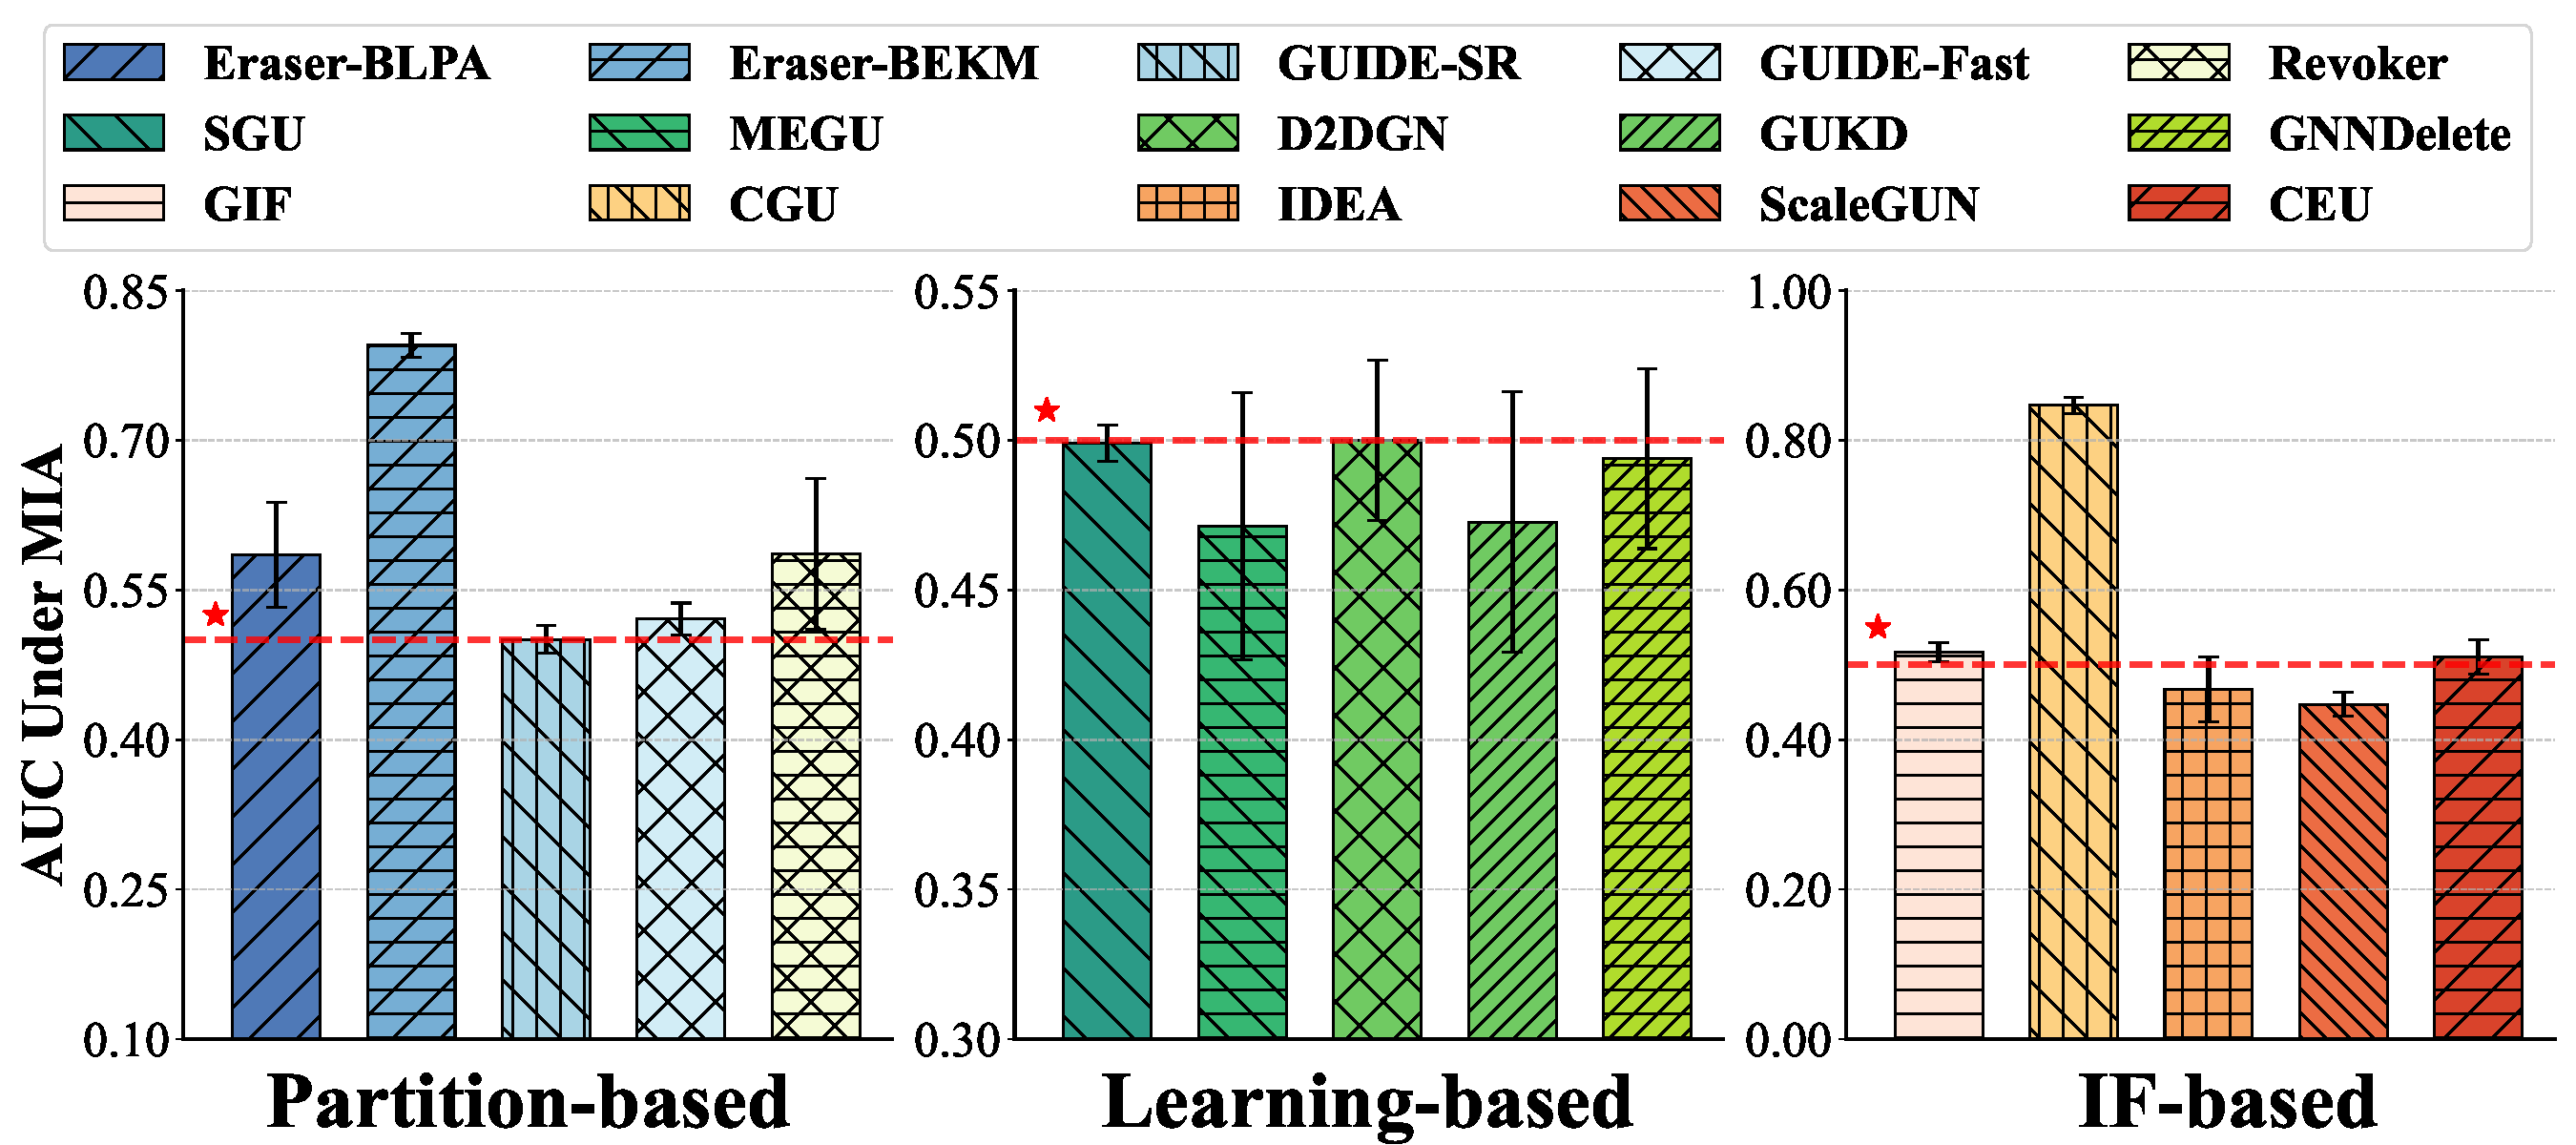
\includegraphics[width=0.5\textwidth]{Pic/Q2MIA_v2.pdf}  % 可根据实际需求调整图片宽度占比
    \caption{AUC-ROC ± STD comparison under MIA for node-node task with SGC backbone.}
    \label{MIA}
    \vspace{-0.3cm}
\end{figure}
\textbf{Graph-Feature Experiment.}
In the current landscape of GU research and OpenGU's integration, GST is the only method proposed to address the GU challenge in graph classification task, highlighting a significant area for further exploration. Given the limited availability of methods tailored to such problems, OpenGU extends existing frameworks and GU strategies to enable graph unlearning in graph classification task, implementing four GU methods. Among these, Partition-based approaches are adapted by extending GraphEraser to the graph classification context, where K-means clustering is used to partition graphs for unlearning. GIF and IDEA, on the other hand, focus on leveraging influence functions to update parameters at the graph level. However, learning-based methods were not adapted as their unlearning strategies are not suitable for graph classification tasks (e.g. lack of node class label). 

We evaluate the performance of these $4$ GU methods on $7$ graph datasets, with the results presented in Table \ref{graph_feature}. The findings reveal that IF-based methods remain effective for graph classification task, achieving commendable performance in most cases. While the Partition-based approach is relatively straightforward, GraphEraser shows competitive performance across these datasets. 
% notably achieving the best performance on the COX2 dataset, surpassing the other three baselines. 
However, GraphEraser faces challenges when applied to large-scale graph, as evidenced by the OOM issue observed on the NCI1 dataset.




% Through the exploration of \textbf{Q1}, we derived two key conclusions. \textbf{C1}: Partition-based methods and GIF-based approaches demonstrate broad applicability across most downstream tasks and unlearning requests. However, Learning-based methods, Projector, and UtU exhibit more specialized strategies, which limit their scalability and generalization. \textbf{C2}: Learning-based methods show significant advantages in tasks focused on predicting remaining nodes within a specific context, often achieving SOTA performance, making them well-suited for targeted tasks. On the other hand, IF-based methods maintain competitiveness in remaining node prediction while offering greater flexibility in their application. 
Through our exploration of \textbf{Q1}, we derive two key conclusions. \textbf{C1}: \textit{Partition and IF-based methods demonstrate broad applicability to most tasks, while Learning-based methods, Projector, and UtU are more specialized, limiting their scalability and generalization} \cite{generalization2,generalization3}. \textbf{C2}: \textit{Learning-based methods excel in targeted tasks, often achieving SOTA performance, while IF-based methods offer flexibility and maintain competitiveness in more tasks} \cite{generalization1}.

\begin{table}[]
\centering
\caption{ACC ± STD comparison(\%) under the setting of graph classification task with feature unlearning. }
\label{graph_feature}
\resizebox{\linewidth}{!}{%
\begin{tabular}{lcccc}
\arrayrulecolor{myblue5}\toprule[0.16em]
\textbf{Graph-Level} & \textbf{GraphEraser}   & \textbf{GST }        &\textbf{ GIF}                     & \textbf{IDEA   }                                \\ \arrayrulecolor{under}\midrule[0.1em]%第二道横线 
MUTAG     & 65.79{\scriptsize \(\pm\)0.05}          & 68.42{\scriptsize \(\pm\)0.13}         & 73.68{\scriptsize \(\pm\)1.03}         & \cellcolor{mycyan!40}\scalebox{0.95}{\textbf{73.68{\scriptsize \(\pm\)0.03}}}         \\
PTC-MR    & 53.04{\scriptsize \(\pm\)0.34}          & 55.07{\scriptsize \(\pm\)0.76}         & 60.29{\scriptsize \(\pm\)2.17}         & \cellcolor{mycyan!40}\scalebox{0.95}{\textbf{60.58{\scriptsize \(\pm\)2.13} }}        \\
BZR       & 73.33{\scriptsize \(\pm\)0.19}          & 74.07{\scriptsize \(\pm\)0.51}         & \cellcolor{mycyan!40}\scalebox{0.95}{\textbf{75.31{\scriptsize \(\pm\)3.02} }}        & 73.33{\scriptsize \(\pm\)4.18}         \\
COX2      & \cellcolor{mycyan!40}\scalebox{0.95}{\textbf{90.21{\scriptsize \(\pm\)0.76} }}         & 88.30{\scriptsize \(\pm\)0.46}         & 88.51{\scriptsize \(\pm\)1.24}         & 87.87{\scriptsize \(\pm\)1.59}         \\
DHRF      & 85.26{\scriptsize \(\pm\)2.68}          & \cellcolor{mycyan!40}\scalebox{0.95}{\textbf{86.18{\scriptsize \(\pm\)3.14} }}        & 74.47{\scriptsize \(\pm\)5.32}         & 67.24{\scriptsize \(\pm\)8.28}         \\
AIDS      & 93.30{\scriptsize \(\pm\)0.10}          & 90.90{\scriptsize \(\pm\)0.20}         & 98.40{\scriptsize \(\pm\)0.12}         & \cellcolor{mycyan!40}\scalebox{0.95}{\textbf{98.50{\scriptsize \(\pm\)0.32} }}        \\
NCI1      & OOM                                    & \cellcolor{mycyan!40}\scalebox{0.95}{\textbf{59.08{\scriptsize \(\pm\)0.20}}}         & 52.90{\scriptsize \(\pm\)1.40}         & 53.63{\scriptsize \(\pm\)1.11}         \\ 
\arrayrulecolor{myblue5}\bottomrule[0.16em]
\end{tabular}}

\end{table}


\begin{figure}[bp]
    \centering
    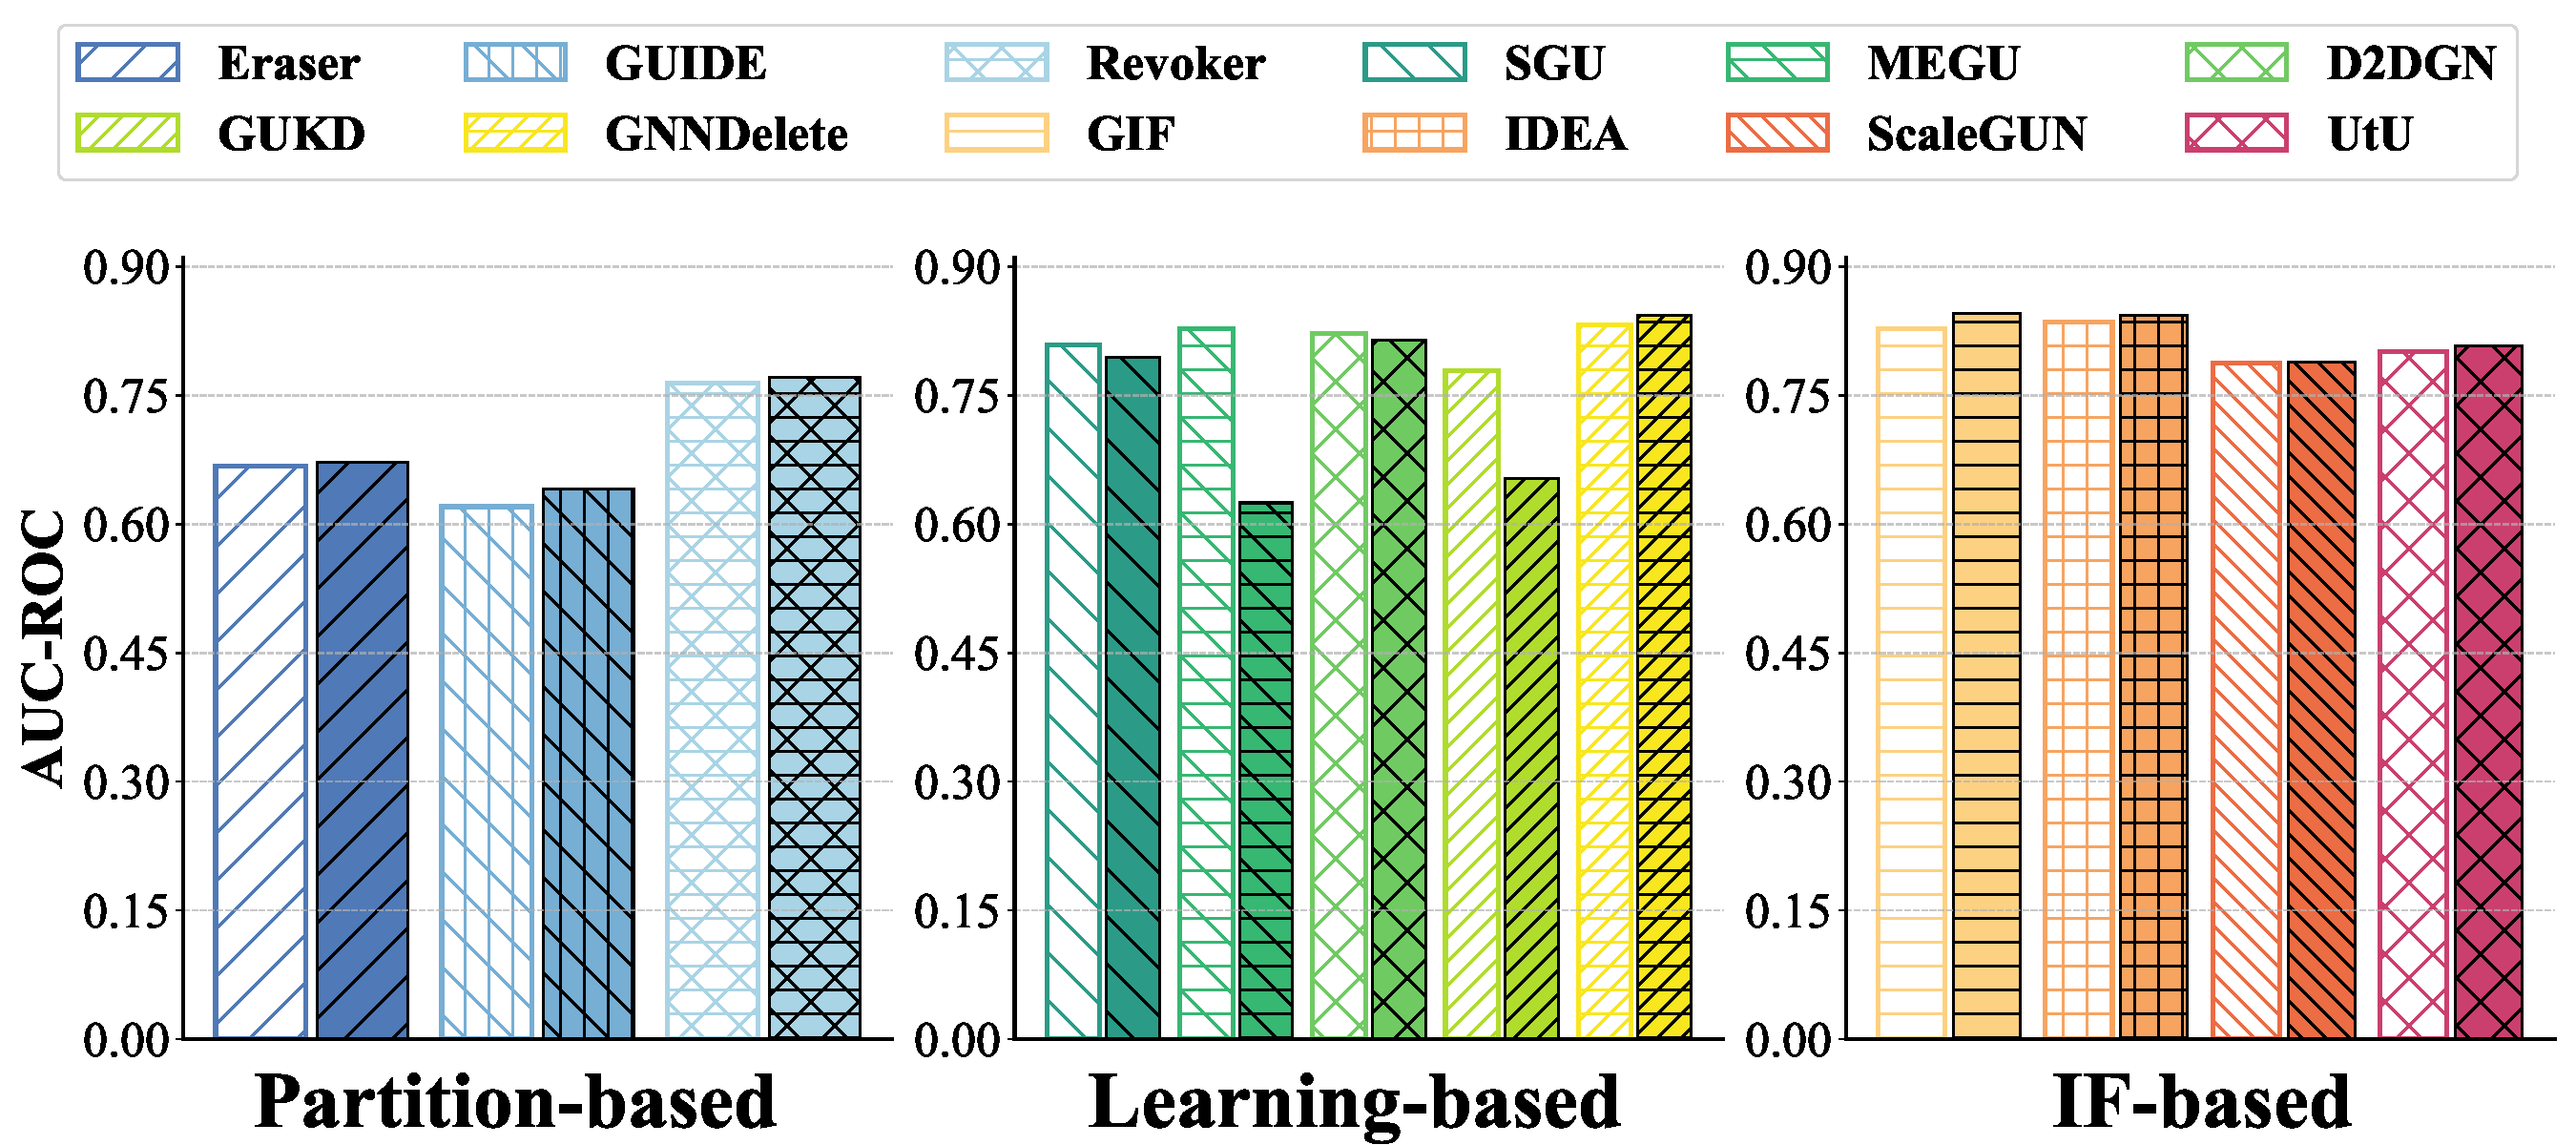
\includegraphics[width=0.5\textwidth]{Pic/Q2Edge_v2.pdf}  % 可根据实际需求调整图片宽度占比
    \caption{AUC-ROC comparison under PA for edge-edge task before and after unlearning with GraphSAGE backbone.}
    \label{Poison}
    \vspace{-0.3cm}
\end{figure}


\subsection{Forgetting Performance Comparison}

To address \textbf{Q2}, we evaluate whether GU algorithms effectively forget the unlearning entity by employing commonly used attack strategies in the GU domain, including Membership Inference Attack and Poisoning Attack. These assessments are conducted from both node and edge perspectives to determine whether existing GU methods can genuinely prevent information leakage and protect privacy. The basic experimental setup is the same as Q1.
% A more detailed explanation of these attack methodologies is provided in Appendix \ref{}.


\begin{figure*}[ht]
    \centering
    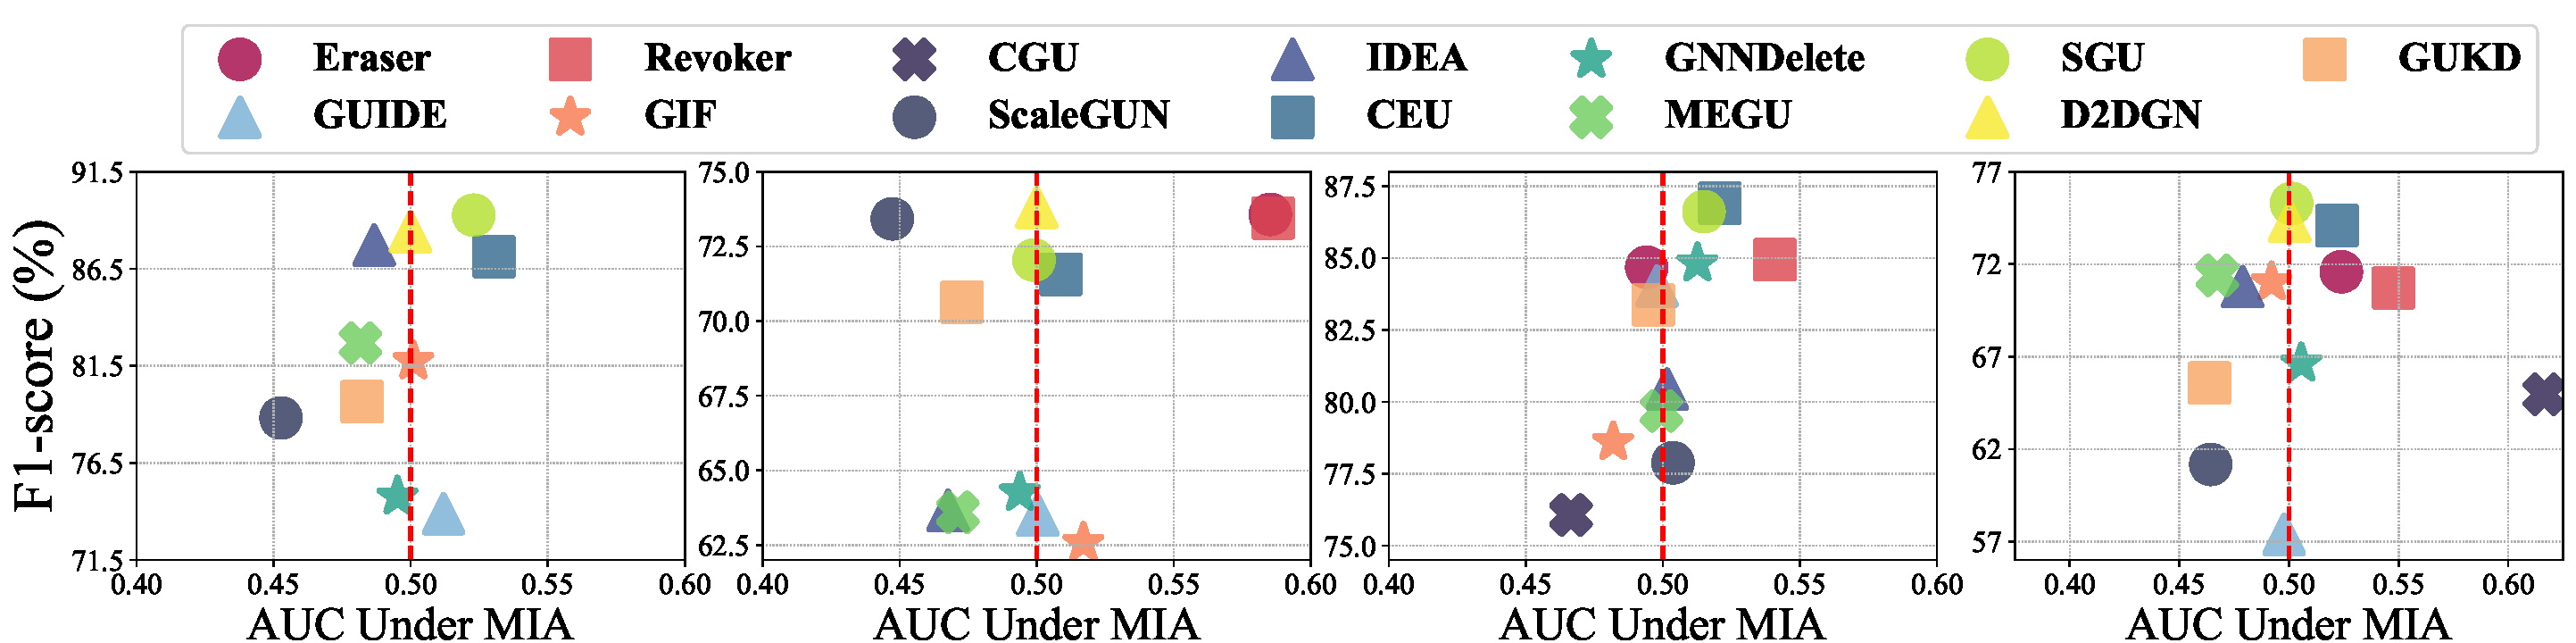
\includegraphics[width=0.95\textwidth]{Pic/Q3_v2.pdf}  % 图片宽度为一栏的一半
    \caption{Trade-off between forgetting and reasoning on Cora, Citeseer, PubMed and in Average performance.}
    \label{Q3}
\end{figure*}

In the node-node experiments, MIA is utilized to assess the extent to which GU algorithms protect model privacy. When the AUC metric approaches 0.5, the predictions become nearly indistinguishable from random guesses, signifying minimal information leakage and thorough removal of sensitive data. To evaluate the performance of various GU methods, we conducted extensive evaluations across multiple datasets and selected the Citeseer dataset as a representative case for result presentation, as shown in Figure \ref{MIA}. The results reveal that: For Partition-based methods, GraphEraser underperforms with the BEKM partitioning strategy, while GUIDE exhibits strong privacy protection when employing SR and Fast partitioning strategies. Among Learning-based methods, SGU, D2DGN, and GNNDelete achieve AUC values close to 0.5, indicating their effectiveness in addressing unlearning requests. Although IF-based methods theoretically analyze and constrain the differences between the original and unlearned models, CGU still falls short of the benchmark for complete unlearning, as evidenced by MIA. 
% Notably, Projector, despite employing a parameter projection strategy to shift to a distinct space, paradoxically increases the risk of information leakage by making MIA more effective at accessing concealed data.





% \begin{figure*}[ht]
%     \centering
%     \begin{minipage}{0.48\textwidth}
%         \centering
%         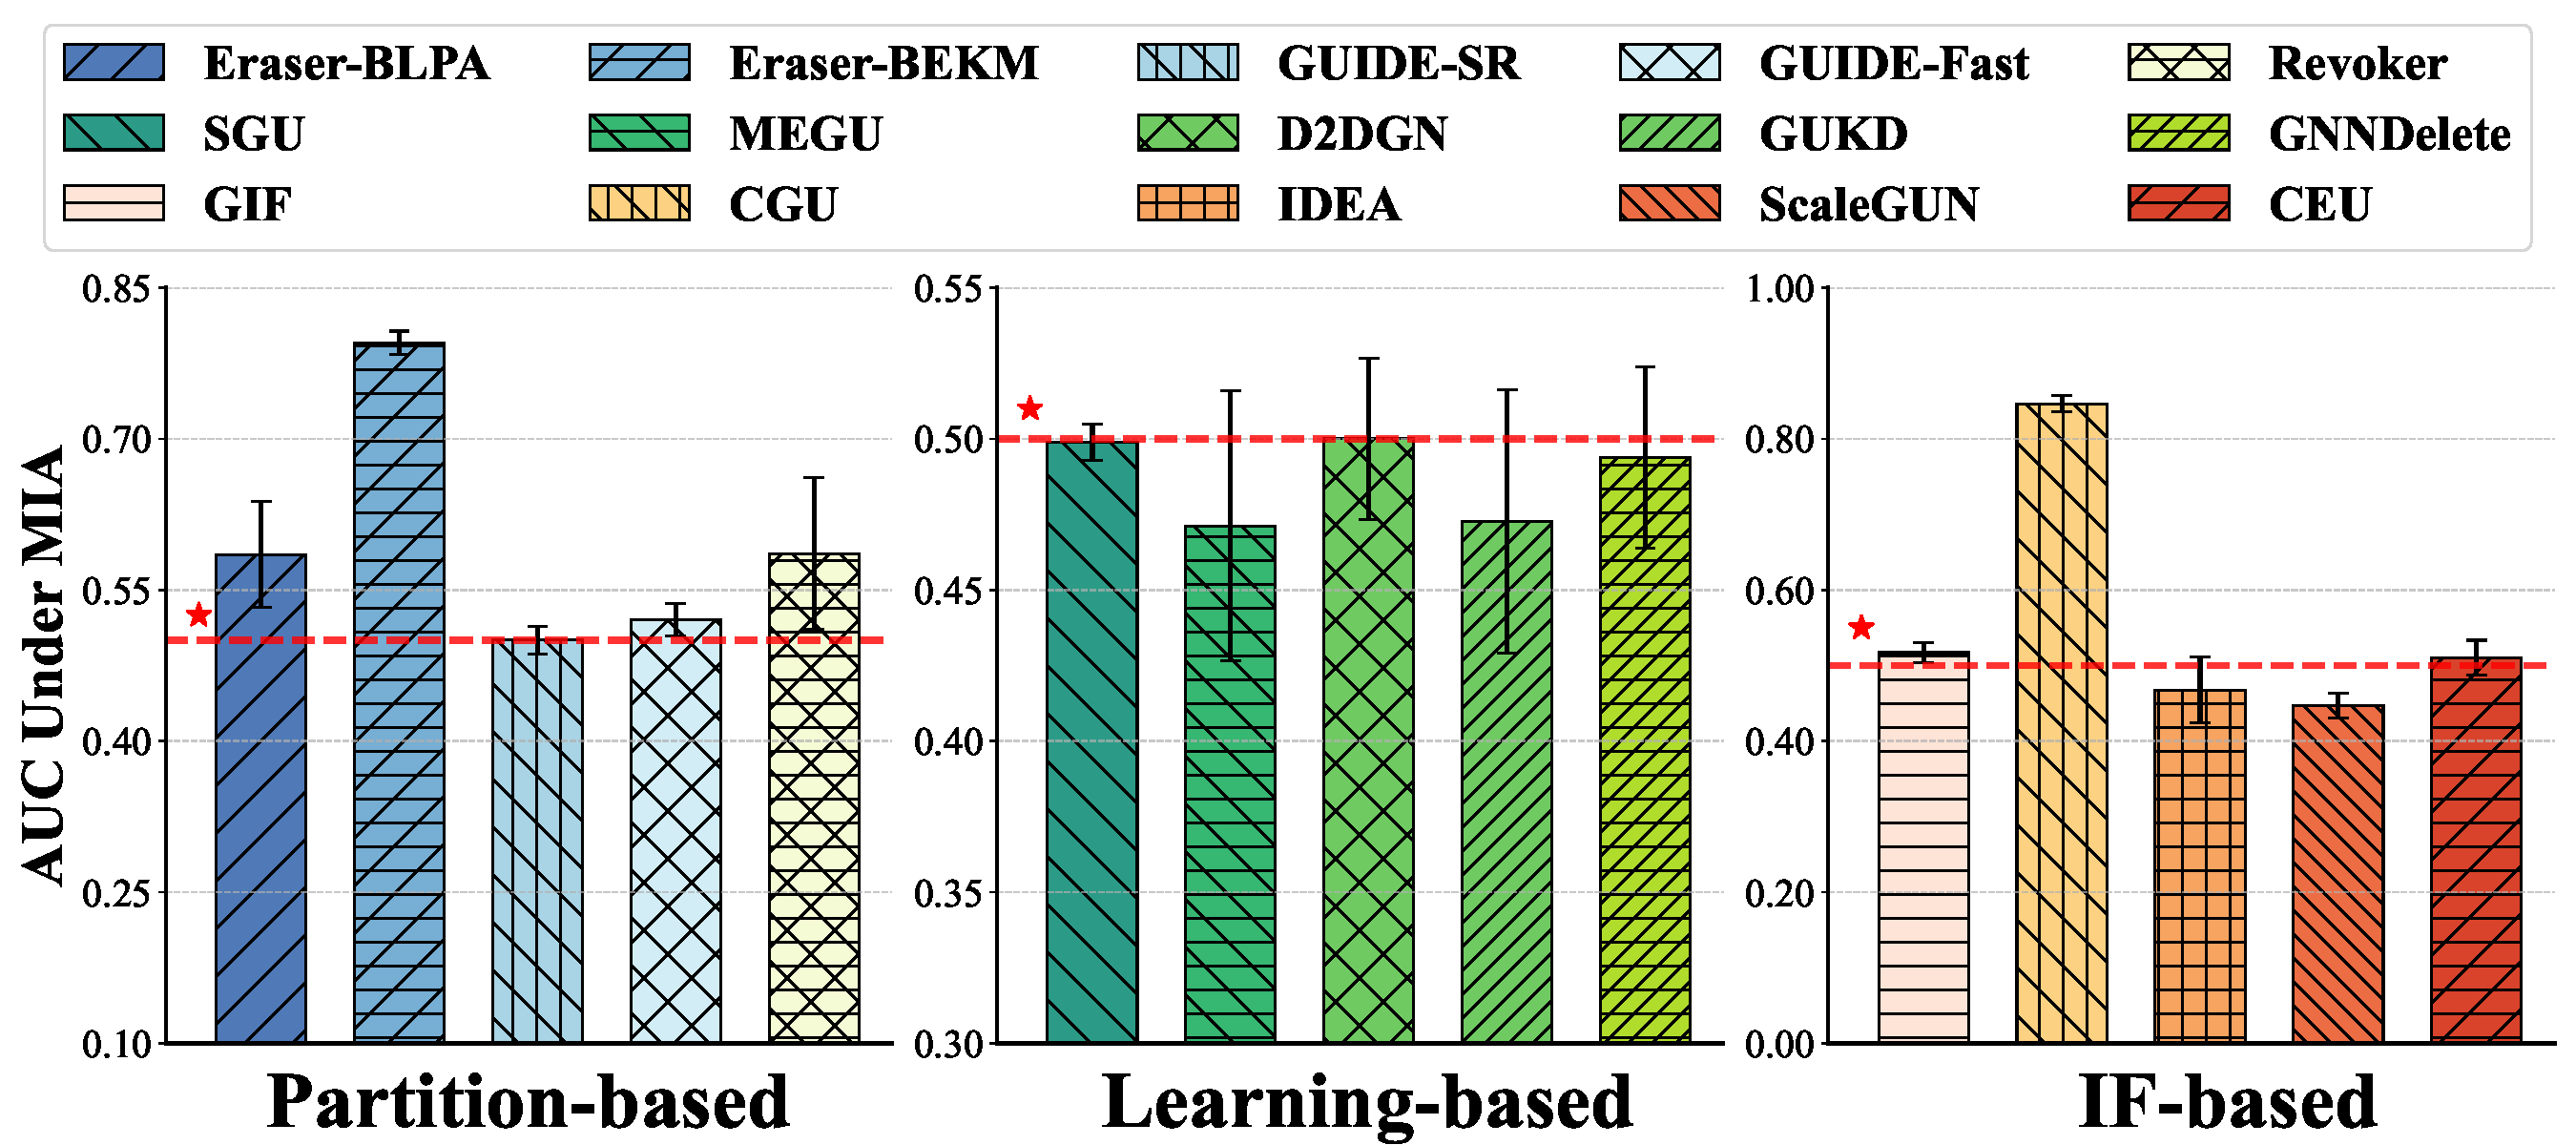
\includegraphics[width=\textwidth]{Pic/Q2MIA.pdf}  % 图片宽度为 minipage 宽度
%         \caption{AUC-ROC ± STD comparison under MIA for node-node task with SGC backbone.}
%         \label{MIA}
%     \end{minipage} \hfill
%     \begin{minipage}{0.48\textwidth}
%         \centering
%         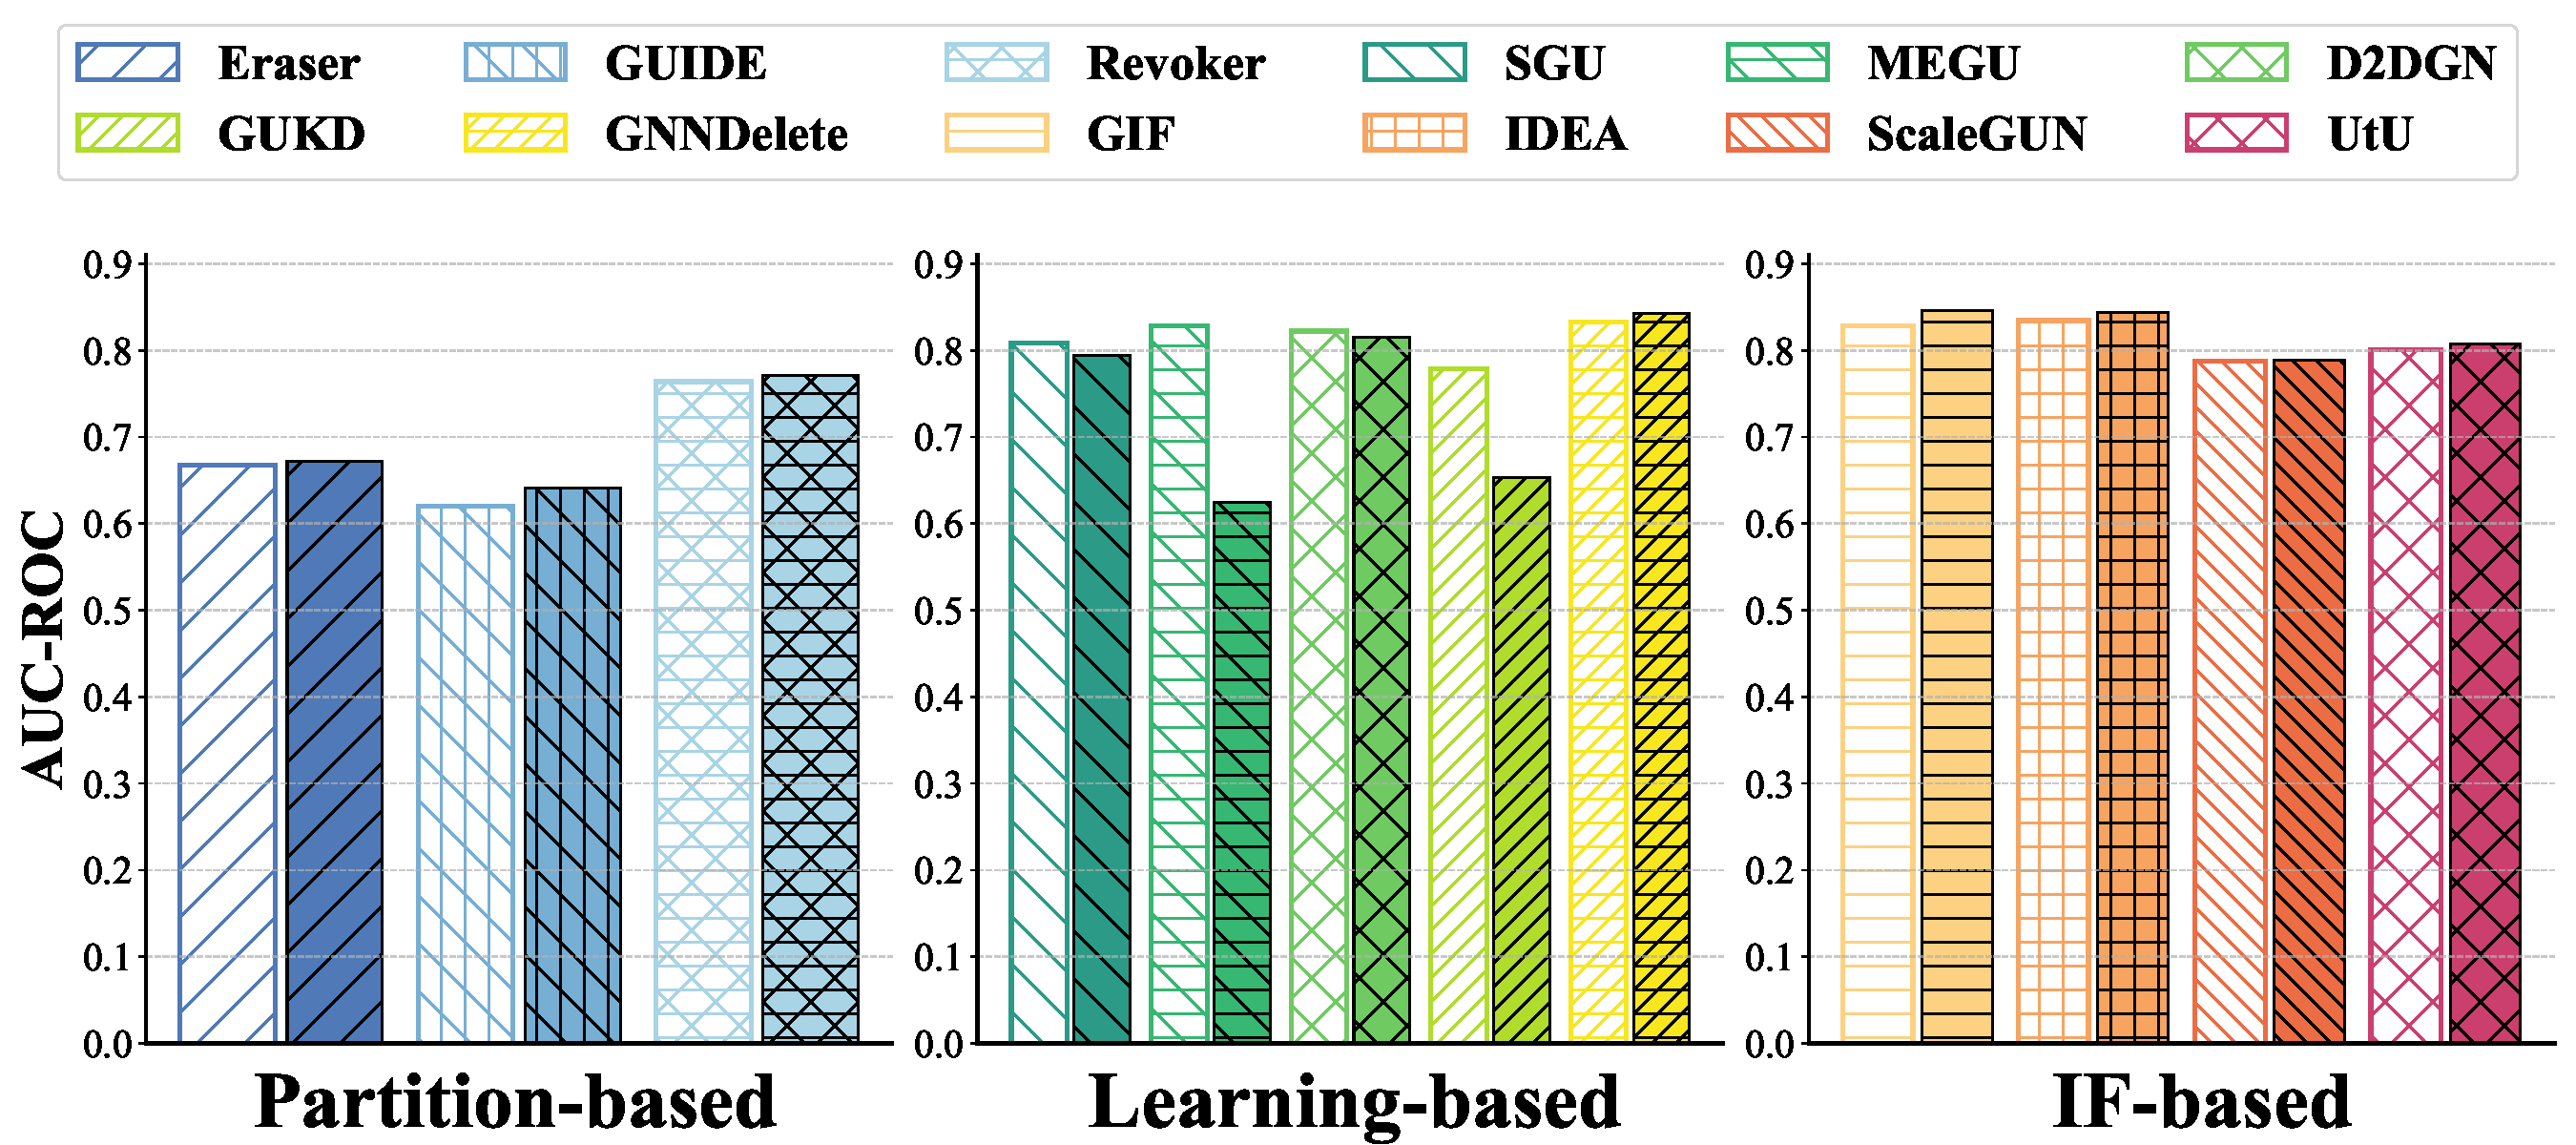
\includegraphics[width=\textwidth]{Pic/Q2Edge.pdf}  % 图片宽度为 minipage 宽度
%         \caption{AUC-ROC comparison under Poisoning Attack for edge-edge task before (Left) and after (Right) unlearning with GraphSAGE backbone. For convenience, UtU is presented in IF-based.}
%         \label{Poison}
%     \end{minipage}
% \end{figure*}





In the edge-edge experiments, we utilized poisoning attack to evaluate the performance of GU methods. Specifically, we selected nodes from different classes and introduced 10\% heterophilic edges, designated as poisoned edges. Intuitively, the addition of these edges disrupts the message-passing mechanism of GNNs, leading to degraded performance on the link prediction task. These poisoned edges are treated as anomalous data and targeted for removal during unlearning. The effectiveness of unlearning is assessed based on the changes in link prediction AUC; a more significant improvement in prediction accuracy after unlearning indicates that the poisoned edge information has been effectively removed.



Extensive experiments are conducted across various datasets. Observations reveal that smaller datasets are more susceptible to the effects of poisoned edges, resulting in more pronounced performance changes. Consequently, we select the Cora dataset, a relatively small dataset, for the presentation of results, as shown in Table \ref{Poison}. For convenience, UtU is presented in IF-based. The findings show that all Partition-based and IF-based methods achieve an increase in AUC after unlearning, demonstrating their capability to address edge-level unlearning requests in link prediction tasks. Among these, GIF and IDEA stand out by not only effectively removing the harmful edges but also achieving high AUC scores, underscoring their robustness. On the other hand, among the Learning-based methods, only GNNDelete successfully handles the removal of poisoned edges during unlearning, achieving a notably high AUC. Other Learning-based approaches exhibit varying levels of performance decline, suggesting that the unlearning process might inadvertently affect critical information. This highlights the significant challenges Learning-based methods face in effectively addressing such scenarios while maintaining model integrity.


Based on our analysis of \textbf{Q2}, we draw the conclusion \textbf{C3}: \textit{Effectiveness of privacy protection in GU methods is more dependent on the strategy design than on the relational categories. There is still significant potential for improvement in maintaining strong unlearning performance across various scenarios} \cite{privacy1,privacy2}.



\vspace{-0.5cm}

\subsection{Trade-off between Forgetting and Reasoning}
To address \textbf{Q3}, we synthesize the insights from the previous two questions and adopt a unified perspective to analyze their interplay.
% synthesize the insights from the previous two questions and 
% examine the trade-off between the reasoning and forgetting capabilities of current GU algorithms. Building on the prior discussions of these capabilities individually, we now take a unified perspective to analyze their interaction. 
Due to space constraints, we focus on the node classification where most GU methods demonstrate strong performance, and utilize SGC as the backbone for consistency across comparisons. To provide a more comprehensive and precise evaluation of the progress achieved by these methods, present the performance of the GU algorithms on Cora, Citeseer, and PubMed respectively. Additionally, we calculate the average performance of the algorithm across nine datasets (consistent with Q1). The summarized results are illustrated in Figure \ref{Q3}, offering a clear overview of the relative performance of different methods in balancing forgetting and reasoning. The methods that are not shown in the figure indicate their AUC exceeds the right boundary.


Given that the most reasonable result of MIA is 0.5, GU methods which are positioned closer to the red centerline and higher up on the graph exhibit superior overall performance. From a vertical perspective, SGU, D2DGN, and CEU excel in reasoning capabilities, whereas GUIDE performs relatively poorly in this regard. From a horizontal perspective, except for CGU, which demonstrates an AUC surpassing 0.6 under MIA, other methods cluster within the range of 0.45 to 0.55. This also indicates the existence of phenomena such as over-forgetting and under-forgetting. Among these, SGU, D2DGN, GNNDelete, and GUIDE manifest robust forgetting capabilities. Notably, while Projector achieves a reasoning performance of approximately 0.68, its approach of projecting weight space into distinct space inadvertently makes sensitive information more accessible to MIA attacks, resulting in an AUC exceeding 0.9. For this reason, Projector is excluded from the comparative visualization. 



Upon exploring \textbf{Q3}, we conclude that \textbf{C4}: \textit{Existing GU algorithms still possess room for enhancement in balancing the trade-off between forgetting and reasoning. The issues of under-forgetting and over-forgetting constitute critical challenges that require further investigation to enhance the overall effectiveness} \cite{tradeoff1,tradeoff2}.


\begin{table*}[t]
\caption{\textbf{Algorithm complexity analysis for existing prevalent GU studies.}}%标题
% \centering%把表居中
% \fontsize{8pt}{9pt}\selectfont% 设置横线宽度
% \setlength{\tabcolsep}{3pt} % 设置列间距
\renewcommand{\arraystretch}{1} % 设置行距
\resizebox{0.95\textwidth}{!}{
\begin{tabular}{l|cccccc}
\arrayrulecolor{myblue5}\toprule[0.16em]

 \textbf{Method}  & \textbf{Preprocessing}  & \textbf{Training} & \textbf{Unlearning}& \textbf{Inference} & \textbf{Memory} \\
 \arrayrulecolor{under}\midrule[0.1em]%第二道横线
 GUIDE         & $ O(ktn^2\!+\!kctn)$            & $O(Lfn/k\!+\!Lf^2n)$         & $O(Lk'fn^2\!/k^2\!+\!Lkf^2n/k)$ & $ O(Lfm\!+\!Lf^2n\!+\!L_kfn)$         & $O(n^2\!/k^2\!+ \!Lfn\! +\! kn)$ \\
GraphEraser   & $O(kdtn\!+\!ktn \!\log(kn))$     & $O(Lfn/k \!+ \!Lf^2n)$         & $O(Lk'\!fn^2/k^2 \!+ \!Lkf^2n/k)$ & $O(Lfm\!+\!Lf^2n\!+\!Ln_{s}f/k \!+\! Ln_{s}f^2)$& $O(n^2\!/k^2 \!+\! Lfn\! + \!kn)$ \\
 GraphRevoker  & $O(k(d+c)n)$                         & $O(Lfn/k \!+\! Lf^2n)$         & $O(Lk'\!fn^2\!/k^2 \!+\! Lkf^2n/k)$ & $O(Lfm\!+\!Lf^2n\!+\!kf^2n_s)$& $O(n^2\!/k^2\! +\! Lfn \!+ \!kn)$ \\ \arrayrulecolor{myblue4}\midrule[0.08em] \addlinespace[-1.5pt] 
\arrayrulecolor{under} \midrule[0.08em]
 GIF           & -                                               & $O(Lfm \!+\! Lf^2n)$           & $O(n|\theta|)$              & $O(Lfm\!+\!Lf^2n)$ & $O(|\theta|)$ \\
 CGU           & -                                             & $O(Lfm \!+\! f^2n)$            & $O((Lmf\! +\! f^2n)u)$           & $O(Lfm\!+\!f^2n)$   & $O(m \!+\! f^2\! +\! fn)$ \\
 CEU           & -                                              & $O(Lfm \!+\! Lf^2n)$           & $O(t|\theta| \!+\! u|\theta|)$   & $O(Lfm\!+\!Lf^2n)$   & $O(|\theta|)$ \\
 GST           & -                                                &   $O(\sum_{i=0}^{N} pg_i^2)$                       & $O(((p\!+\!|\theta|)\!\sum_{i=0}^{N}g_i^2\!+\!|\theta|^3)u)$        & $O(\sum_{i=0}^{N} pg_i^2)$  & $O(pfn)$ \\
 IDEA          & -                                                & $O(Lfm\!+\!Lf^2n)$                         & $O(n|\theta|)$          & $O(Lfm\!+\!Lf^2n)$ & $O(|\theta|)$ \\
 ScaleGUN      & -                      & $O(Lfm\!+\!f^2n)$       & $O(L^2d^2u)$                          &  $O(Lfm\!+\!f^2n)$ 
  &$O(m\!+\!f^2\!+\!fn)$\\ \arrayrulecolor{myblue4}\midrule[0.08em] \addlinespace[-1.5pt] 
\arrayrulecolor{under} \midrule[0.08em]
 SGU           &$O(Bf^2 \!+\! Bn_s \!+\! f^2u)$                                             & $O(Lfm \!+ \!f^2n)$            & $O(Lf^2\!+\!Bn_sf\!+\!(c\!+\!f)u)$     & $O(Lfm \!+\! f^2n)$  & $O(Bfn_s \!+\! f^2)$ \\
 MEGU          & $O(Lfm \!+ \!Lf^2n\!+\!d^2u)$                                             & $O(Lfm \!+ \!Lf^2n \!+ \!d^2u)$            &  $O(d^2cu)$     & $O(Lfm \!+\! Lf^2n)$ & $O(Lfm \!+ \!f^2n)$ \\
 GUKD          &   $O(Lfm\!+\!Lf^2n)$                                             &$O(L_t fm\!+\!Lf^2n)$                        & $O(c(n\!-\!u))$                     & $O(Lfm \!+\! Lf^2n)$  & $O(f^2\!+\!fn)$\\
 D2DGN         &       $O(Lfm\!+\!Lf^2n)$                    &  $O(Lfm\!+\!Lf^2n) $                     &              $O(c(n\!-\!u))$         & $O(Lfm \!+\! Lf^2n)$  & $O(f^2\!+\!fn)$ \\
 GNNDelete     & $O(Lfm\! +\! Lf^2n \!+\!d^2u)$                                             & $O(Lfm \!+\! Lf^2n)$             & $O(d^2fu)$ & $O(Lfm \!+\! Lf^2n)$ & $O(fu \!+ \!d^2\!fu)$ \\ \arrayrulecolor{myblue4}\midrule[0.08em] \addlinespace[-1.5pt] 
\arrayrulecolor{under} \midrule[0.08em]
 Projector     & -                                             & $O(Lfm \!+\! Lf^2n)$           & $O(f^2n \!+\! \max\{u^3\!, \!f^2u\})$ & $O(Lfm \!+\! Lf^2n)$  & $O(f^2 \!+ \!fn)$ \\
 UtU           & -                                             & $O(Lfm \!+\! Lf^2n)$                          & $O(u)$                        & $O(Lfm \!+\! Lf^2n)$  & $O(m \!+\! Lfn)$ \\ 
 \arrayrulecolor{myblue5}\bottomrule[0.16em]
\end{tabular}%
}
\label{complex}
\vspace{-0.15cm}
\end{table*}



\vspace{-1.5em}
\subsection{Algorithm Complexity Analyses}
To answer \textbf{Q4} about how the GU algorithms perform in terms of time and space complexity, we analyze the time complexity from the perspectives of preprocessing, training, unlearning, and inference. Since partition-based methods are unique, their partitioning is included in the preprocessing, while aggregation is incorporated into inference.
% Given that partition-based methods are unique, the partitioning part of such algorithms is included in the preprocess section, and the aggregation part is incorporated into the inference section.
Additionally, we provide a comprehensive summary of the space complexity for all methods, encompassing the required memory for model parameters, data storage, and auxiliary structures, ensuring a thorough evaluation. Except for the methods that can only act on edge-level, we take node unlearning as the perspective of analysis. The results are presented in Table \ref{complex}.




For clarity in the complexity analysis, we introduce a set of key notations that will be used consistently throughout the discussion. To ensure a uniform evaluation of complexity, we consider GCN as the backbone model, with the number of layers denoted by $L$. In terms of the dataset, $n$ represents the total number of nodes, $m$ refers to the number of edges, $f$ is the feature dimension of the nodes, and $d$ denotes the average degree of the nodes. The number of classes is denoted by $c$, 
% which corresponds to the label dimensionality, 
while $u$ signifies the number of unlearning requests, representing the nodes, edges or features to be deleted during the unlearning process. 
Since part of the methods involve sampling, we define the number of samples as $n_s$.



For \textbf{Partition-based} methods, the parameter $k$ represents the number of shards, 
% into which the graph is divided, 
and $t$ denotes the number of iterations required by the algorithm. For the three methods considered, the fundamental approach is similar, leading to comparable time and space complexities in both the training and unlearning phases. The principal differences between these GU methods are manifested in the partitioning and aggregation. In the partitioning phase, GUIDE and GraphEraser depend on non-training algorithms, whereas GraphRevoker relies on constructing loss functions. During the aggregation phase, GUIDE utilizes the pyramid match graph kernel, with complexity $ O(L_kfn)$, where $L_k$ is the number of layers in the kernel.


% For most \textbf{IF-based} methods, the training time is primarily bounded by $O(Lfm+Lf^2n)$. Specifically, in the case of GST, 
% % , which is designed for graph-level classification tasks, 
% the initialization time complexity is expressed as $O(\sum_{i=0}^{N} pg_i^2)$. Here, $N$ is the number of graphs, $g_i$ denotes the number of nodes in graph $G_i$, and $p$ corresponds to $O(\sum_{l=0}^{L-1} J^l)$ determined by the $J$-ary scattering tree. Regarding the unlearning process, since these methods utilize influence function for analysis, the unlearning complexity and memory overhead are predominantly dependent on the model parameter $\theta$. 
% For ScaleGUN, the paper indicates that the time complexity for removing a single edge is approximately $O(L^2d)$. When considering node unlearning, the time complexity is constrained by $O(L^2d^2u)$.
For \textbf{IF-based} methods, the unlearning process relies on influence function, where the time and memory complexity are primarily determined by the model parameters $\theta$. These methods often optimize by approximating the inverse of the Hessian matrix, which typically requires a complexity of $O(|\theta|^3)$. In the case of GST, the initialization time is expressed as $O(\sum_{i=0}^{N} pg_i^2)$, where $N$ is the number of graphs, $g_i$ denotes the node number in graph $G_i$, and $p$ corresponds to $O(\sum_{l=0}^{L-1} J^l)$ determined by the $J$-ary scattering tree.


For \textbf{Learning-based} methods, the training phase typically involves training the GNNs
% on the entire dataset, 
with the time complexity bounded by $O(Lfm + Lf^2n)$. In the case of GUKD, an additional step is required to train a teacher model, which may differ in layer depth from the target model. To account for this difference, we define the layer count of the teacher model as $L_t$.
% Moreover, since most Learning-based GU methods rely on sampling or similar operations to enhance efficiency, the unlearning process introduces complexity terms influenced by the number of unlearning requests $u$, the sampling size $n_s$, or hyperparameters such as $B$ in SGU. 
The memory complexity of Learning-based GU methods varies depending on their specific design and operations. For example, SGU leverages node influence maximization strategies, resulting in a memory complexity of $O(Bfn_s \!+\! f^2)$, where $B$ stands for the budget hyperparameter. 
% GNNDelete's memory usage is primarily determined by the neighborhood of the edges involved in the unlearning process, leading to a complexity of $O(fu\!+\!d^2fu)$.

% For Projector, the authors employed a specialized algorithm to simplify the matrix inversion process, ultimately limiting the time complexity to $O(f^2n \!+\! \max\{u^3\!, \!f^2u\})$, with the space complexity controlled at $O(f^2 \!+ \!fn)$. Notably, for UtU, since it only alters the graph's information without requiring additional training, the unlearning process incurs negligible time overhead $O(u)$, being primarily dependent on the number of deletion requests.
Based on the analysis, we conclude \textbf{C5}: \textit{To reduce time costs, partition-based methods require optimization in partitioning, IF-based methods need to minimize the computational overhead of Hessian matrix calculations in specific GU scenarios, and learning-based approaches demand enhanced efficiency in the preprocessing} \cite{Efficient1,Efficient2}.




\begin{figure*}[ht]
    \centering
    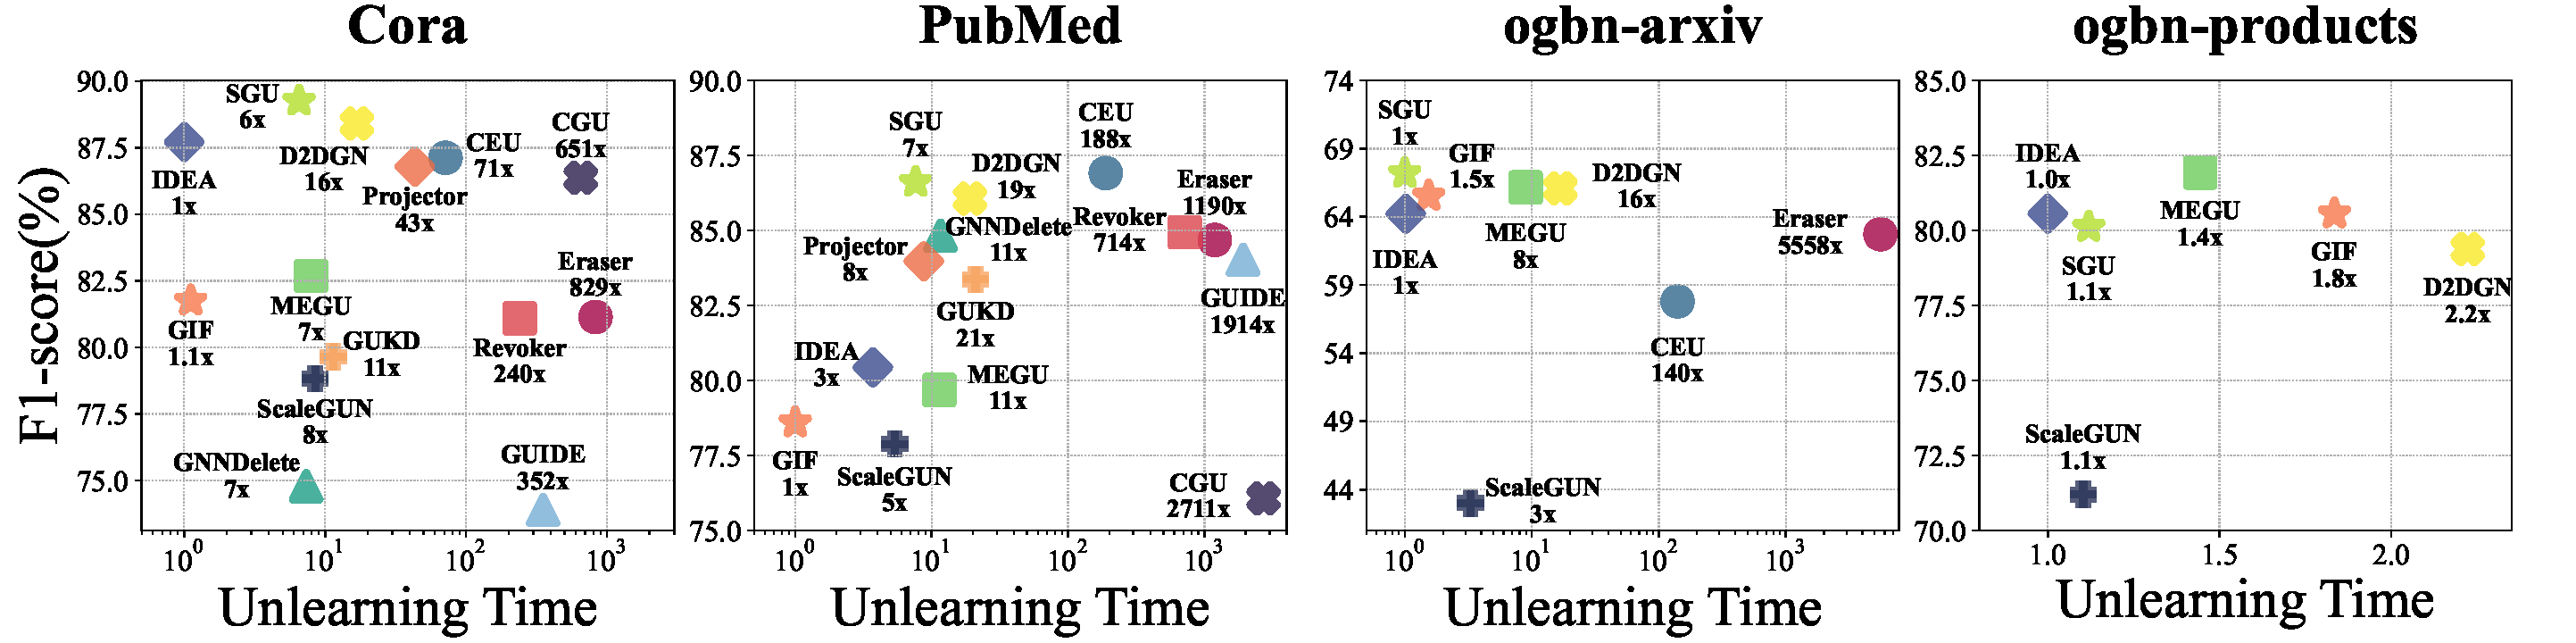
\includegraphics[width=0.97\textwidth]{Pic/Q5_f1_time_v2.pdf}  % 图片宽度为一栏的一半
    \vspace{-0.1cm}
    % \caption{Unlearning Time Performance on Diverse Datasets with  Increasing Scale.}
    \caption{Unlearning Time Performance on Cora, PubMed, ogbn-arxiv and ogbn-products.}
    \label{Q5_time}
    \vspace{-0.1cm}
\end{figure*}
    \vspace{-0.1cm}
\begin{figure*}[ht]
    \centering
    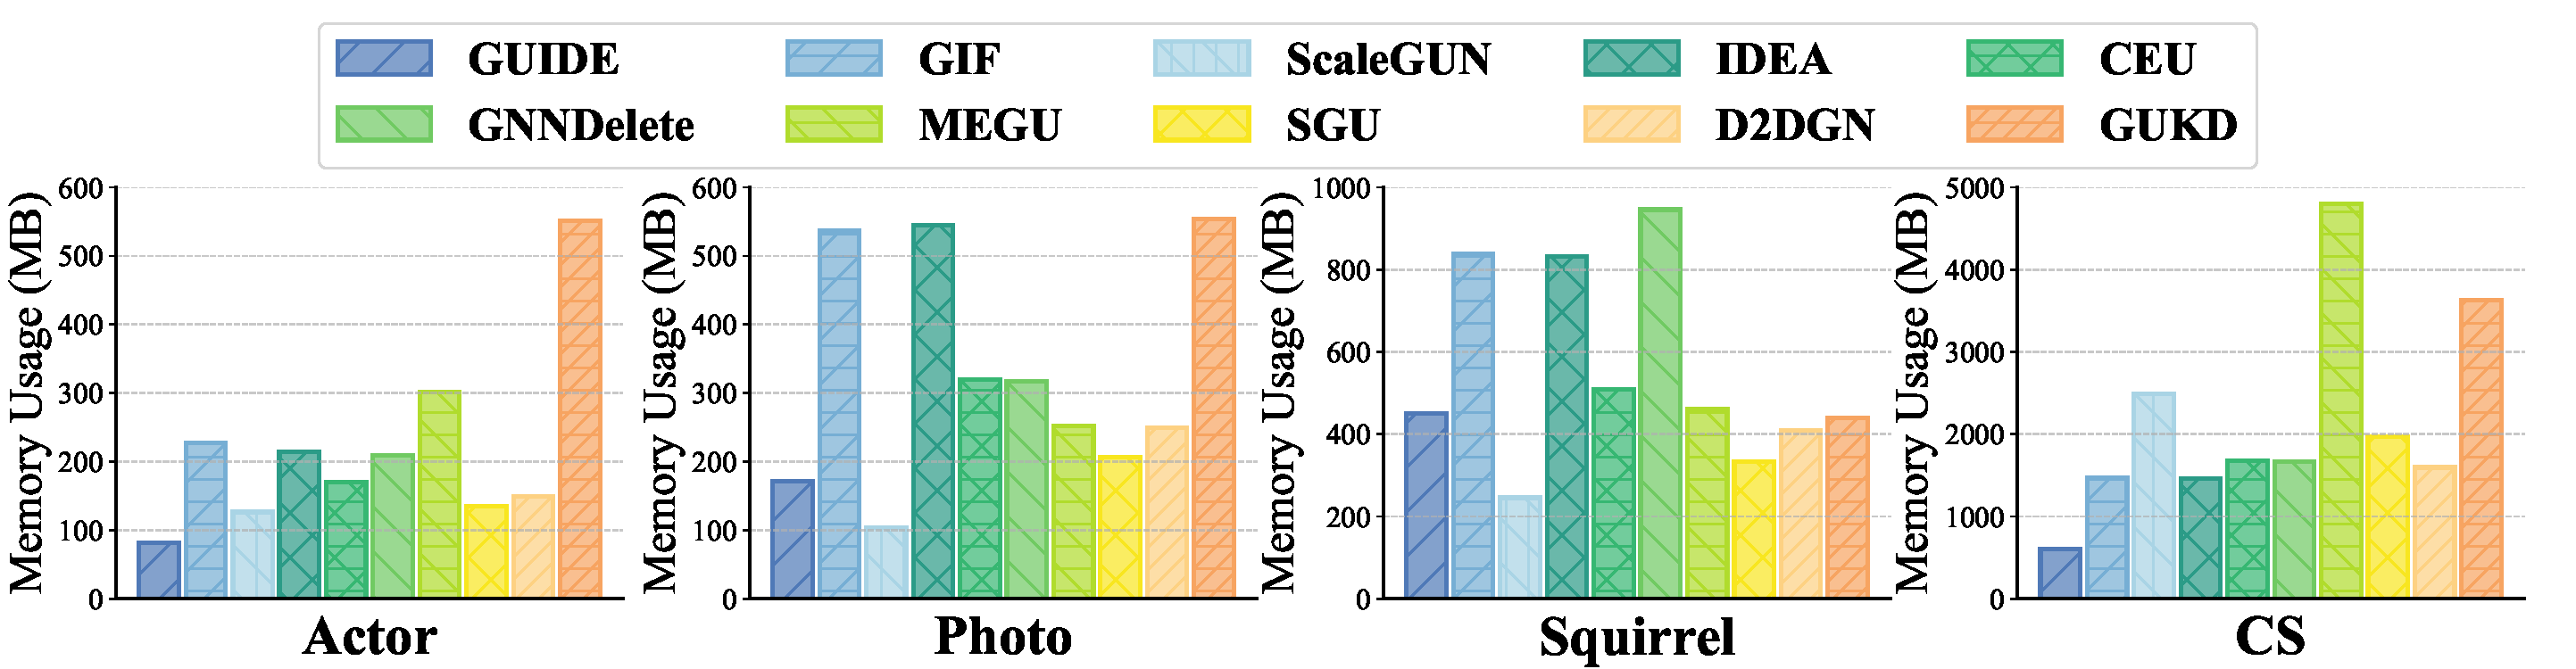
\includegraphics[width=0.97\textwidth]{Pic/Q5_mem.pdf}  % 图片宽度为一栏的一半
    \vspace{-0.1cm}
    \caption{Memory Usage Performance on Various Datasets.}
    \label{Q5_mem}
    \vspace{-0.1cm}
\end{figure*}




\subsection{Practical Efficiency Analyses}
In addressing \textbf{Q5}, we evaluated the time and memory overhead of GU algorithms under a 10\% node unlearning request on a range of datasets, with a focus on the node classification. As depicted in Figure \ref{Q5_time}, we selected four datasets of increasing scale, from the small Cora dataset with thousands of nodes to the large-scale ogbn-products dataset with millions of nodes, to ensure a fair comparison in terms of time cost and scalability. Partition-based methods display substantial time overhead on account of partitioning, aggregation, and shard training operations, whereas most IF-based and Learning-based methods exhibit greater temporal efficiency. On large-scale datasets like ogbn-products, only $6$ GU methods were able to run, with comparable performance, while others faced challenges such as timeouts or memory overflows. Regarding memory usage in Figure \ref{Q5_mem}, GUIDE consistently exhibits low memory overhead across various datasets, while GraphEraser (without visualization) incurs considerably higher costs, exceeding 4000MB even on smallest dataset Actor. Notably, methods that are capable of handling large datasets, such as ScaleGUN and SGU, maintain stable memory consumption across all datasets, thereby demonstrating their scalability. 

Based on our analysis, we conclude \textbf{C6}: \textit{Existing GU methods require further optimization to effectively reduce time and space overhead, emphasizing the need for more efficient implementations in both computation and memory usage} \cite{Efficient3,Efficient4}.

\subsection{Impact of Unlearning Intensity}
To address Q6, we conducted node unlearning experiments on Cora and ogbn-arxiv and edge unlearning experiments on Citeseer and Chameleon, employing various backbones for the node classification task. The unlearning ratio was incrementally increased from 0 to 0.5, and the results are presented in Figure \ref{Q6_ratio}. The illustration reveals a consistent downward trend in performance for all GU methods as the unlearning ratio increases, indicating that higher deletion intensities negatively impact prediction capabilities. Notably, methods such as Projector, GIF, and CEU exhibit greater sensitivity to changes in certain datasets, while Learning-based methods demonstrate a more gradual decline, highlighting their robustness under higher unlearning intensities. However, we also observe that even with minimal deletion ratios, many methods experience significant performance degradation during unlearning, particularly on the Chameleon dataset. This suggests that current GU algorithms need to take the deletion ratio into account to better reduce the gap in predictive performance between the unlearned and original model. Based on this analysis, we derive conclusion \textbf{C7}: \textit{While most GU algorithms perform reasonably well across varying unlearning intensities, there remains a critical need to enhance their robustness across diverse datasets} \cite{robustness1}.


\begin{figure*}[ht]
    \centering
    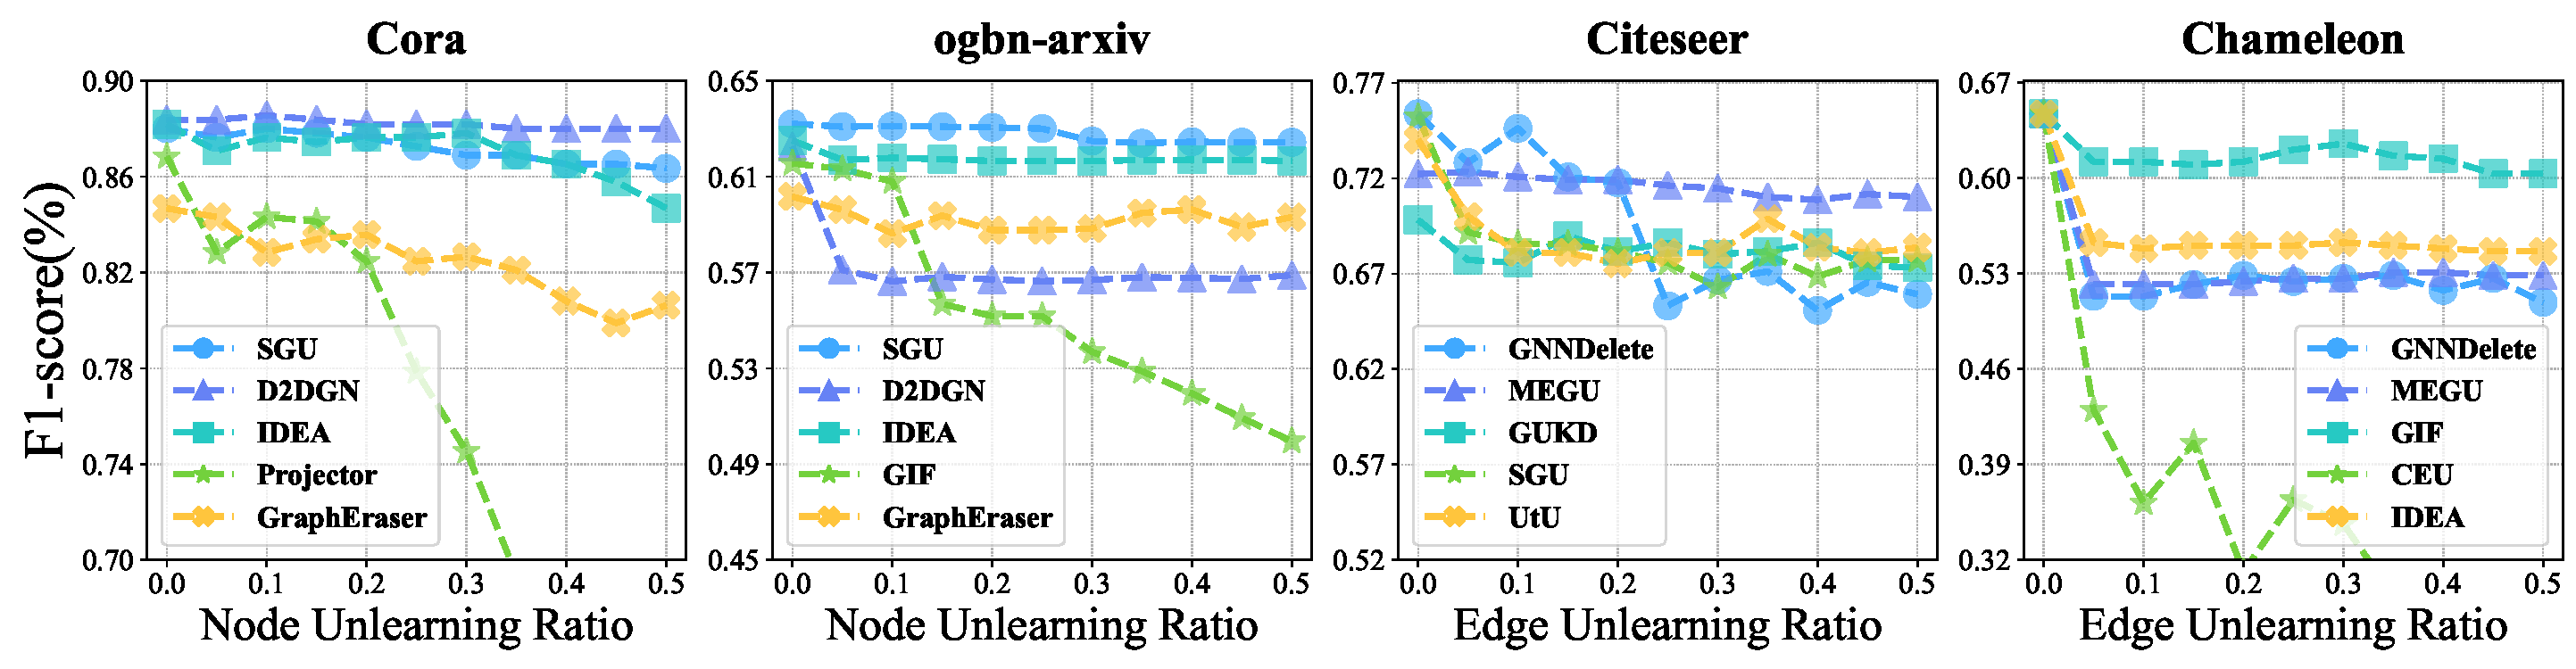
\includegraphics[width=1\textwidth]{Pic/Q6_unlearn_ratio_3.pdf}  % 图片宽度为一栏的一半
    \caption{Performance under Different Unlearning Intensities with GraphSAINT, Cluster-gcn, GAT, and GCN.}
    \label{Q6_ratio}
\end{figure*}


\begin{figure*}[ht]
    \centering
    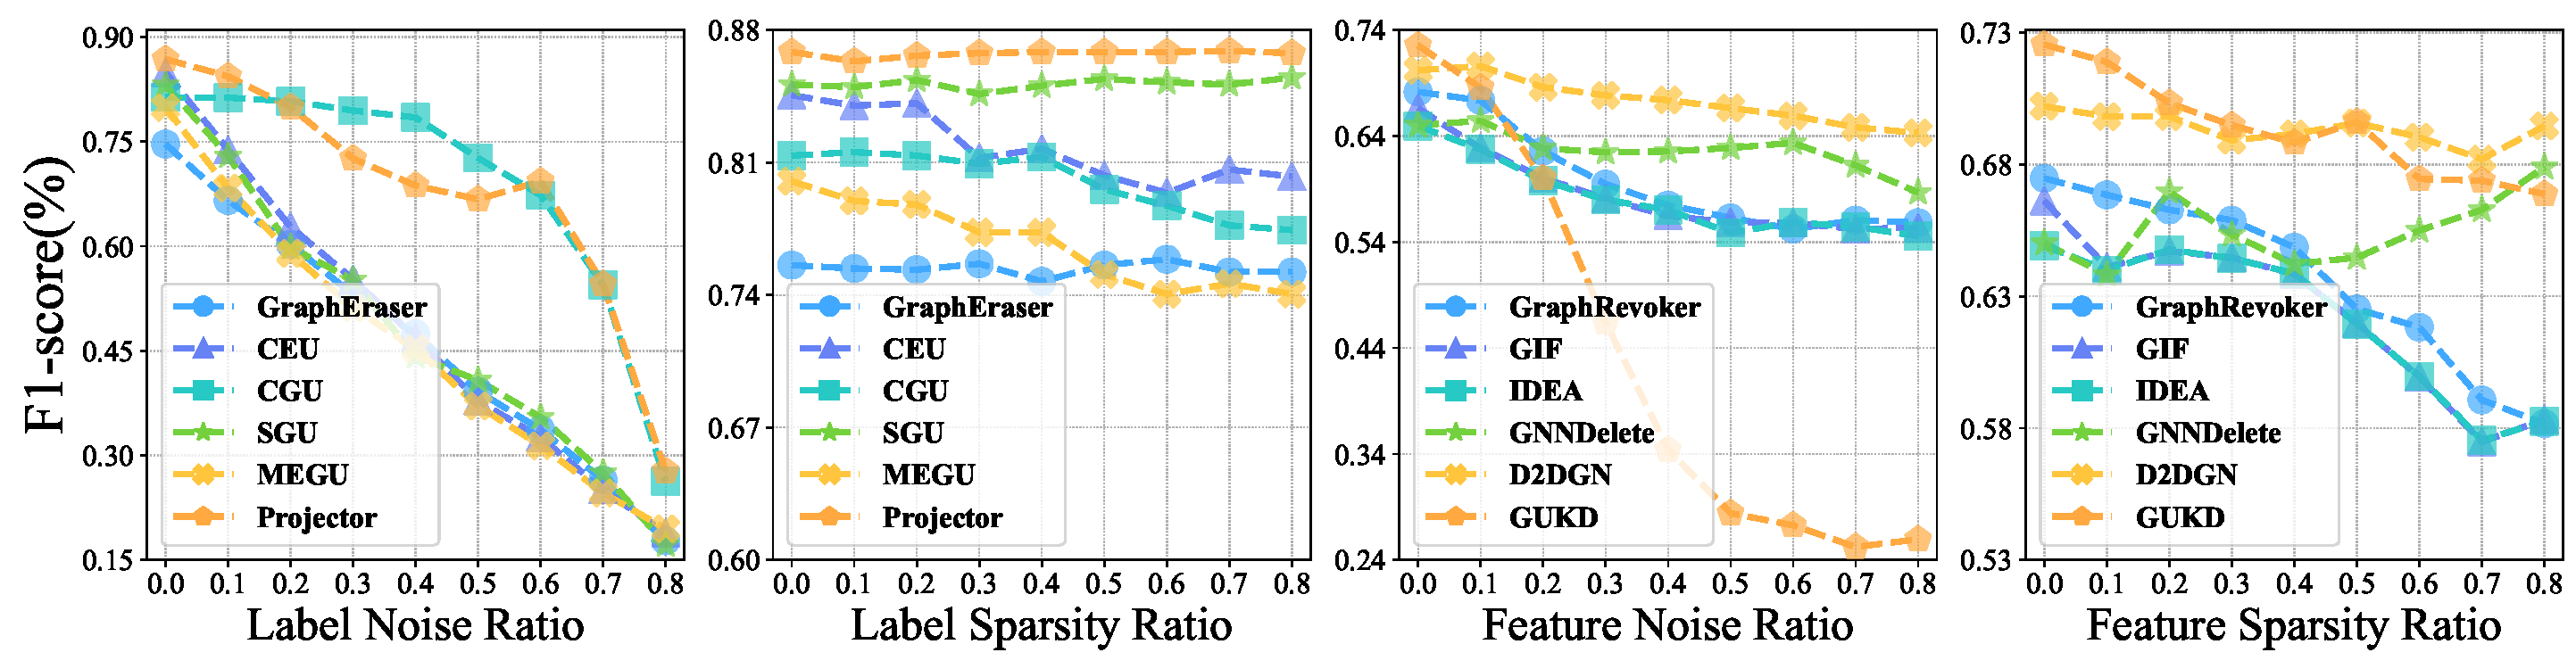
\includegraphics[width=1\textwidth]{Pic/Q7_robustness.pdf}  % 图片宽度为一栏的一半
    \caption{Performance under Different Noise and Sparsity Ratios at Label and Feature Levels.}
    \label{Q7}
\end{figure*}
\subsection{Robustness Analyses}
To address \textbf{Q7}, we simulate more realistic noise and sparsity scenarios by introducing perturbations at both the label and feature levels to comprehensively evaluate the robustness of existing GU methods. For label noise, a certain proportion of training samples are randomly assigned incorrect labels, while for feature noise, Gaussian noise is injected based on the dimensionality of node features. Sparsity is introduced by varying the proportion of training nodes and simulating partial feature absence. Given the large number of GU methods, we select representative approaches for analysis based on their categories, using the same settings as the node-node experiments in Q1 and adopting SSGC as the backbone. The results, presented in Figure \ref{Q7}, reveal that nearly all methods experience a decline in predictive performance under the influence of noise and sparsity, with label noise exerting the most pronounced impact. Specifically, CGU and Projector exhibit a pattern of slow initial degradation followed by a rapid decline, while other methods demonstrate a steady and sharp drop. When the noise ratio reaches 0.8, the F1-score for all methods falls below 0.3. In contrast, the impact of label sparsity is comparatively minor, with some methods even maintaining their original performance. Under feature noise, GUKD experiences a significant performance drop, indicating its limited resilience to feature perturbations. For feature sparsity, methods like GIF, IDEA, and GraphRevoker show marked declines, whereas GNNDelete surprisingly improves. These findings lead us to conclude \textbf{C8}: \textit{Current GU methods exhibit insufficient robustness to noise and sparsity, particularly in the presence of label noise, which poses a significant challenge to enhancing the overall robustness of GU approaches} \cite{robustness2}.


% \begin{figure*}[ht]
%     \centering
%     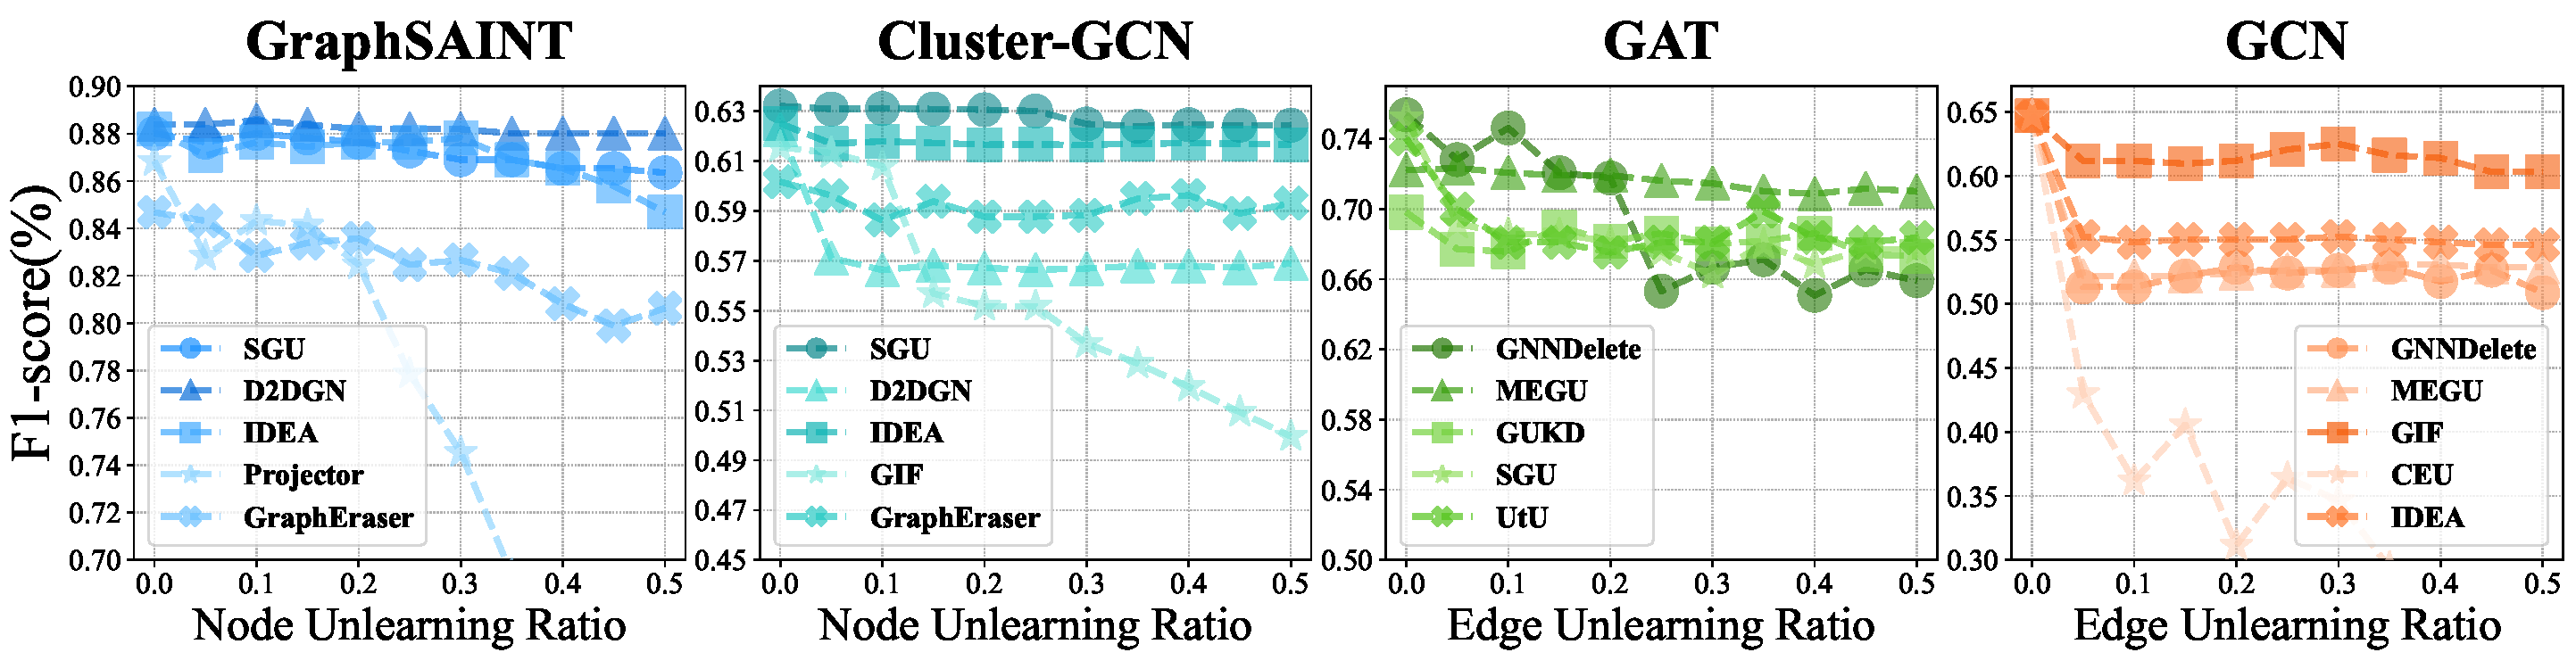
\includegraphics[width=1\textwidth]{Pic/Q6_unlearn_ratio.pdf}  % 图片宽度为一栏的一半
%     \caption{unlearnratio}
%     \label{Q6_ratio}
% \end{figure*}



% Please add the following required packages to your document preamble:
% \usepackage{multirow}
% \usepackage{graphicx}




% Backbone & GU method &Cora &Citeseer & PubMed &ogbn-arxiv &CS & Flickr &Chameleon &Minesweeper & Tolokers\\
% \midrule%第二道横线 
% \multirow{10}{*}{GCN}&GraphEraser & 82.05±0.91    & 74.20±0.77 & 86.10±0.15 & 59.95±0.11& 92.08±0.05 & 49.35±0.14 & 50.09±0.51 & 80.72±0.10 & \underline{79.55±0.20}\\
% \multirow{10}{*}{}   &GUIDE       & 82.93±1.79    & 67.47±1.45 & 85.71±0.28 & OOM        & 88.66±0.16 & {\color{red}8.51±0.03} & 38.05±0.94 & {\color{red}44.71±0.00} & {\color{red}44.11±0.00}\\
% \multirow{10}{*}{}   &GraphRevoker& 82.34±1.79    & 74.23±0.49 & 86.20±0.16 & 59.96±0.11 & 91.97±0.05 & 49.33±0.17 & 49.74±0.80 & 80.77±0.08 & \textbf{79.66±0.08}\\
% \multirow{10}{*}{}   &GIF         & 85.83±0.59    & 68.68±0.61 & 83.87±0.17 & 63.86±0.49 & 93.02±0.30 & 49.71±0.05 & 61.10±0.74 & 80.40±0.38 & 79.09±0.47\\
% \multirow{10}{*}{}   &IDEA        & 88.12±0.28    & 68.44±0.29 & 84.06±0.22 & 59.57±0.30 & \underline{93.73±0.16} & 44.78±0.79 & 53.68±1.33 & 80.04±0.41 & 74.73±2.38\\
% \multirow{10}{*}{}   &GNNDelete   & 74.80±3.77    & 65.62±4.19 & 81.00±2.25 & OOM & 65.06±4.24 & 42.03±0.00 & 43.51±1.40 & \textbf{80.87±0.02} & 79.07±0.12\\  
% \multirow{10}{*}{}   &MEGU        & 85.30±0.66    & 68.02±2.34 & 83.15±1.20 & \underline{64.90±0.42} & 91.95±0.20 & 48.79±0.18 & 60.48±0.99 & 80.54±0.38 & 79.06±0.10\\
% \multirow{10}{*}{}   &SGU         & \textbf{94.17±0.41} & 74.92±0.25 & \textbf{88.62±0.04} & \textbf{65.50±0.43} & \textbf{94.26±0.06} & \textbf{51.17±0.04} & \underline{66.97±0.41} &\underline{80.85±0.00} & 79.28±0.02\\
% \multirow{10}{*}{}   &D2DGN       & \underline{89.06±0.32}& \underline{75.17±0.65} & \underline{88.00±0.11} & 62.39±0.40 & 93.29±0.07 & \underline{50.86±0.07} & \textbf{67.24±0.69} & 80.84±0.02 & 79.29±0.04\\
% \multirow{10}{*}{}   &GUKD        & 83.06±1.84    &70.78±1.79 & 84.52±0.47 & OOM & {\color{red}15.41±6.15} & 42.03±0.12 & {\color{red}30.57±2.84} & 80.85±0.00 & 78.91±0.00\\ \midrule


% \multirow{11}{*}{SGC}&GraphEraser & 81.14±1.00    & 73.57±1.25 & 84.68±0.54 & 62.72±0.18 & 91.24±0.08 & 46.93±0.14 & 45.18±1.46 & 80.45±0.08 & 78.36±0.30\\
% \multirow{11}{*}{}   &GUIDE       & 73.89±2.18    & 63.50±0.71 & 84.02±0.15 & OOM        & 86.96±0.15 & {\color{red}8.48±0.02} & {\color{red}18.86±4.37} & {\color{red}44.71±0.00} & {\color{red}44.11±0.00}\\
% \multirow{11}{*}{}   &GraphRevoker& 81.09±1.63    & 73.45±0.61 & 84.94±0.14 & 62.72±0.18 & 91.26±0.10 & 46.91±0.14 & 44.87±1.72 & 80.44±0.12 & 78.36±0.30\\
% \multirow{11}{*}{}   &GIF         & 81.75±1.09    & 62.58±0.67 & 78.60±0.22 & 65.52±0.17 & 91.87±0.22 & 47.56±0.12 & \underline{55.09±1.23} & 77.83±0.09 & 78.44±0.10\\
% \multirow{11}{*}{}   &CGU         & 86.37±0.78    & \textbf{75.62±0.41} & 76.07±0.15 & OOT & OOT & OOT & {\color{red}35.83±0.74} & {\color{red}43.90±2.53} & {\color{red}26.22±1.49}\\
% \multirow{11}{*}{}   &IDEA        & 87.71±0.25    & 63.66±0.49 & 80.44±0.13 & 64.22±0.17 & 89.47±0.22 & 42.01±0.04 & 52.89±0.80 & 77.93±0.04 & 78.72±0.15\\
% \multirow{11}{*}{}   &GNNDelete   & 74.78±5.49    & 64.26±3.82 & 84.82±1.36 & OOM & 76.26±2.73 & 42.03±0.00  & 54.43±1.87 & 81.04±0.19 & 79.12±0.16\\
% \multirow{11}{*}{}   &MEGU        & 82.68±1.56    & 63.60±1.11 & 79.68±0.60 & \underline{66.15±0.29} & 91.69±0.08 & 47.97±0.13 & 53.82±1.68 & 77.64±0.02 & \textbf{79.29±0.10}\\
% \multirow{11}{*}{}   &SGU         & \textbf{89.26±0.49}& 72.04±1.70 & \textbf{86.61±0.02} & \textbf{67.20±0.08} & \textbf{93.20±0.07} & \textbf{48.70±0.21} & \textbf{60.18±0.26} &\underline{81.11±0.02} & \underline{79.18±0.04}\\
% \multirow{11}{*}{}   &D2DGN       & \underline{88.41±0.20} & \underline{73.81±0.28} & \underline{86.06±0.05} & 66.08±0.18 & \underline{92.99±0.03} & \underline{48.01±0.03} & 53.25±0.70 & \textbf{81.19±0.04} & 79.18±0.05\\
% \multirow{11}{*}{}   &GUKD        & 79.65±1.98    & 70.63±0.93 & 83.37±0.60 & OOM & {\color{red}28.33±6.57} & 42.03±0.04 & {\color{red}33.42±2.50} & 80.89±0.04 & 78.91±0.00\\ \midrule

% ADGCN &Projector  &86.79±2.37 & \textbf{77.00±0.65} & 83.97±0.30 & OOT & 88.40±0.63 & OOT & 43.29±1.17 & 80.85±0.00 & 78.91±0.00\\
% GST   & GST       &75.72±0.97 & 73.40±0.60 & 73.40±0.61 & {\color{red}23.40±0.09} & 68.39±0.44 & 42.05±0.02 & {\color{red}23.95±3.31} & {\color{red}21.26±1.48} & {\color{red}27.36±0.72}\\

\vspace{-0.3cm}